%%Initial Setup
%%  A simple AAU report template.
%  2014-09-13 v. 1.1.0
%  Copyright 2010-2014 by Jesper Kjær Nielsen <jkn@es.aau.dk>
%
%  This is free software: you can redistribute it and/or modify
%  it under the terms of the GNU General Public License as published by
%  the Free Software Foundation, either version 3 of the License, or
%  (at your option) any later version.
%
%  This is distributed in the hope that it will be useful,
%  but WITHOUT ANY WARRANTY; without even the implied warranty of
%  MERCHANTABILITY or FITNESS FOR A PARTICULAR PURPOSE.  See the
%  GNU General Public License for more details.
%
%  You can find the GNU General Public License at <http://www.gnu.org/licenses/>.
%
% \documentclass[12pt,twoside,a4paper,openright]{report}
\documentclass[12pt,twoside,a4paper,openany]{report}
%%%%%%%%%%%%%%%%%%%%%%%%%%%%%%%%%%%%%%%%%%%%%%%%
% Language, Encoding and Fonts
% http://en.wikibooks.org/wiki/LaTeX/Internationalization
%%%%%%%%%%%%%%%%%%%%%%%%%%%%%%%%%%%%%%%%%%%%%%%%
% Select encoding of your inputs. Depends on
% your operating system and its default input
% encoding. Typically, you should use
%   Linux  : utf8 (most modern Linux distributions)
%            latin1 
%   Windows: ansinew
%            latin1 (works in most cases)
%   Mac    : applemac
% Notice that you can manually change the input
% encoding of your files by selecting "save as"
% an select the desired input encoding. 
\usepackage[utf8]{inputenc}
% Make latex understand and use the typographic
% rules of the language used in the document.
\usepackage[danish,english]{babel}

%% ssary things
%\usepackage[acronym]{glossaries}
%\makeglossaries




% Use the palatino font
\usepackage[sc]{mathpazo}
\linespread{1.05}         % Palatino needs more leading (space between lines)
% Choose the font encoding
\usepackage[T1]{fontenc}
%%%%%%%%%%%%%%%%%%%%%%%%%%%%%%%%%%%%%%%%%%%%%%%%
% Graphics and Tables
% http://en.wikibooks.org/wiki/LaTeX/Importing_Graphics
% http://en.wikibooks.org/wiki/LaTeX/Tables
% http://en.wikibooks.org/wiki/LaTeX/Colors
%%%%%%%%%%%%%%%%%%%%%%%%%%%%%%%%%%%%%%%%%%%%%%%%
% load a colour package
%%TEMP REMOVED!!!!!!!%%%%%\usepackage{xcolor}
\usepackage[pdftex,dvipsnames]{xcolor}
\definecolor{aaublue}{RGB}{33,26,82}% dark blue
% The standard graphics inclusion package
\usepackage{graphicx}
\graphicspath{{Pictures/}}
% Set up how figure and table captions are displayed
\usepackage{caption}
\captionsetup{%
  font=footnotesize,% set font size to footnotesize
  labelfont=bf % bold label (e.g., Figure 3.2) font
}
\usepackage{subcaption}
% Make the standard latex tables look so much better
\usepackage{array,booktabs}
% Enable the use of frames around, e.g., theorems
% The framed package is used in the example environment
\usepackage{framed}

%%%%%%%%%%%%%%%%%%%%%%%%%%%%%%%%%%%%%%%%%%%%%%%%
% Mathematics
% http://en.wikibooks.org/wiki/LaTeX/Mathematics
%%%%%%%%%%%%%%%%%%%%%%%%%%%%%%%%%%%%%%%%%%%%%%%%
% Defines new environments such as equation,
% align and split 
\usepackage{amsmath}
% Adds new math symbols
\usepackage{amssymb}
% Use theorems in your document
% The ntheorem package is also used for the example environment
% When using thmmarks, amsmath must be an option as well. Otherwise \eqref doesn't work anymore.
\usepackage[framed,amsmath,thmmarks]{ntheorem}

%%%%%%%%%%%%%%%%%%%%%%%%%%%%%%%%%%%%%%%%%%%%%%%%
% Page Layout
% http://en.wikibooks.org/wiki/LaTeX/Page_Layout
%%%%%%%%%%%%%%%%%%%%%%%%%%%%%%%%%%%%%%%%%%%%%%%%
% Change margins, papersize, etc of the document
\usepackage[
	left=15mm,
	right=15mm,
	top=2cm,
	bottom=3cm
	%left=15mm,
	%right=15mm,
	%top=3cm,
	%bottom=3cm
	]{geometry} 
% Modify how \chapter, \section, etc. look
% The titlesec package is very configureable
\usepackage{titlesec}
%\titleformat{\chapter}[display]{\normalfont\huge\bfseries\color{aaublue}}{\chaptertitlename\ \thechapter}{20pt}{\Huge}
\titleformat*{\section}{\normalfont\Large\bfseries\color{aaublue}}
\titleformat*{\subsection}{\normalfont\large\bfseries\color{aaublue}}
\titleformat*{\subsubsection}{\normalfont\normalsize\bfseries\color{aaublue}}
%\titleformat*{\paragraph}{\normalfont\normalsize\bfseries\color{aaublue}}
%\titleformat*{\subparagraph}{\normalfont\normalsize\bfseries\color{aaublue}}

% Clear empty pages between chapters
\let\origdoublepage\cleardoublepage
\newcommand{\clearemptydoublepage}{%
  \clearpage
  {\pagestyle{empty}\origdoublepage}%
}
\let\cleardoublepage\clearemptydoublepage
% Tools to flip page content (tables, pictures, etc.)
\usepackage{adjustbox}
\usepackage{rotating}
% Adjustable table width/height structure
\usepackage{tabularx}
\usepackage[vlines]{tabularht}
% Change the headers and footers
\usepackage{fancyhdr}
\pagestyle{fancy}
\usepackage[Sonny]{fncychap}
\fancyhf{} %delete everything
\renewcommand{\headrulewidth}{0pt} %remove the horizontal line in the header
\fancyhead[RE]{\color{aaublue}\small\nouppercase\leftmark} %even page - chapter title
\fancyhead[LO]{\color{aaublue}\small\nouppercase\rightmark} %uneven page - section title
\fancyhead[LE,RO]{\thepage} %page number on all pages
\setlength{\headheight}{14.5pt} 
% Do not stretch the content of a page. Instead,
% insert white space at the bottom of the page
\raggedbottom
% Enable arithmetics with length. Useful when
% typesetting the layout.
\usepackage{calc}

%%%%%%%%%%%%%%%%%%%%%%%%%%%%%%%%%%%%%%%%%%%%%%%%
% Bibliography
% http://en.wikibooks.org/wiki/LaTeX/Bibliography_Management
%%%%%%%%%%%%%%%%%%%%%%%%%%%%%%%%%%%%%%%%%%%%%%%%
% Add the \citep{key} command which display a
% reference as [author, year]
\usepackage[numbers]{natbib}
% Appearance of the bibliography
\bibliographystyle{plainnat}

%%%%%%%%%%%%%%%%%%%%%%%%%%%%%%%%%%%%%%%%%%%%%%%%
% Misc
%%%%%%%%%%%%%%%%%%%%%%%%%%%%%%%%%%%%%%%%%%%%%%%%
% Include full pdf pages
\usepackage{pdfpages}
% Add bibliography and index to the table of
% contents
\usepackage[nottoc]{tocbibind}
% Add the command \pageref{LastPage} which refers to the
% page number of the last page
\usepackage{lastpage}
% Add todo notes in the margin of the document
\usepackage[
%  disable, %turn off todonotes
colorinlistoftodos, %enable a coloured square in the list of todos
textwidth=\marginparwidth, %set the width of the todonotes
%textsize=scriptsize, %size of the text in the todonotes
]{todonotes}

%%%%%%%%%%%%%%%%%%%%%%%%%%%%%%%%%%%%%%%%%%%%%%%%
% Hyperlinks
% http://en.wikibooks.org/wiki/LaTeX/Hyperlinks
%%%%%%%%%%%%%%%%%%%%%%%%%%%%%%%%%%%%%%%%%%%%%%%%
% Enable hyperlinks and insert info into the pdf
% file. Hypperref should be loaded as one of the 
% last packages
\usepackage{hyperref}
\hypersetup{%
	%pdfpagelabels=true,%
	plainpages=false,%
	pdfauthor={Livia Elena Anghel, Raul Cos, Felix Gravila, Vojtech Jindra, Valer Orlovsky, Miroslav Pakanec},%
	pdftitle={Passenger Classification},%
	pdfsubject={Passenger Classification},%
	pdfkeywords={AAU project 7 semester Passenger Classification Blip System},%
	bookmarksnumbered=true,%
	colorlinks,%
	citecolor=aaublue,%
	filecolor=aaublue,%
	linkcolor=aaublue,% you should probably change this to black before printing
	urlcolor=aaublue,%
	pdfstartview=FitH%
}
\newenvironment{itquote}
  {\begin{quote}\itshape}
  {\end{quote}\ignorespacesafterend}
\usepackage{listings}
\usepackage{float}
\usepackage{wrapfig}
%\usepackage{subfig}
\usepackage{url}

%%\usepackage{minted}
%\definecolor{graa}{rgb}{0.9, 0.9, 0.9}
%\usepackage{tcolorbox}
%\tcbuselibrary{minted,skins}
%\newtcblisting{mintedboks}[1]{
%	listing engine=minted,
%	colback=graa,
%	colframe=black!70,
%	listing only,
%	minted style=colorful,
%	minted language=#1,
%	minted options={
%	    linenos=true,
%	    tabsize=4,
%        texcl=true,
%		fontsize=\footnotesize,
%		numbersep=3mm,
%		breaklines=true,
%		fontfamily=tt
%	},
%	top=-0.5mm,
%	bottom=-0.5mm,
%	left=5mm,
%	enhanced,
%	overlay={\begin{tcbclipinterior}\fill[black!25] (frame.south west)
%	  		rectangle ([xshift=5mm]frame.north west);\end{tcbclipinterior}}
%}

\expandafter\def\expandafter\UrlBreaks\expandafter{\UrlBreaks%  save the current one
  \do\a\do\b\do\c\do\d\do\e\do\f\do\g\do\h\do\i\do\j%
  \do\k\do\l\do\m\do\n\do\o\do\p\do\q\do\r\do\s\do\t%
  \do\u\do\v\do\w\do\x\do\y\do\z\do\A\do\B\do\C\do\D%
  \do\E\do\F\do\G\do\H\do\I\do\J\do\K\do\L\do\M\do\N%
  \do\O\do\P\do\Q\do\R\do\S\do\T\do\U\do\V\do\W\do\X%
  \do\Y\do\Z}

%No indent  
\newlength\tindent
\setlength{\tindent}{\parindent}
\setlength{\parindent}{0pt}
\renewcommand{\indent}{\hspace*{\tindent}}

%\usepackage{etoolbox}
%\makeatletter
%\patchcmd{\FV@SaveLineBox}{%
%	\strut#1\strut
%}{%
%\hyphenchar\font=%
%% Invisible hyphen:
%\if\expandafter\@car\f@encoding\relax\@nil O 255 \else 23 \fi
%% Visible hyphen:
%% `\- %
%\strut
%\nobreak % prevent line break by next \hspace
%\hspace{0pt}% allow hyphenation of first word
%#1%
%\nobreak % without the following \strut would prevent hyphenation of previous word
%\strut
%}{}{%
%\errmessage{\noexpand\FV@SaveLineBox could not be patched}%
%}
\makeatother
\usepackage[linesnumbered]{algorithm2e}
%\usepackage{msctexen}
\usepackage{color}

\usepackage[footnote,draft,silent,nomargin]{fixme}
\fxsetup{theme=color}
%\definecolor{fxtarget}{rgb}{255,0.0000,0.0000}

%Use cleverref
\usepackage[english]{cleveref}

%include eps file extensions
\usepackage{epstopdf}
\epstopdfsetup{outdir=./epsfigs/}

% Forskellige muligheder for todo's
\newcommand{\unsure}[1]{\todo[linecolor=red,backgroundcolor=red!25,bordercolor=red,inline]{LÆS! #1}\mbox{}}
\newcommand{\change}[2][1=]{\todo[linecolor=yellow,backgroundcolor=yellow!25,bordercolor=yellow,#1]{#2}}
\newcommand{\info}[1]{\todo[linecolor=blue,backgroundcolor=blue!25,bordercolor=blue,inline]{#1}}
\newcommand{\missingref}[1]{\todo[linecolor=Magenta,backgroundcolor=Magenta!25,bordercolor=Magenta]{\textbf{Mangler ref!} #1}}
\newcommand{\missingcite}[1]{\todo[linecolor=Magenta,backgroundcolor=Magenta!25,bordercolor=Magenta]{\textbf{Mangler kilde!} #1}}
\newcommand{\missingdesc}[1]{\todo[linecolor=Magenta,backgroundcolor=Magenta!25,bordercolor=Magenta]{\textbf{Mangler beskrivelse!} #1}}

% Sætter hvor mange tal der skal gives ud og hvor mange der skal vises i indholdsfortegnelse
\setcounter{tocdepth}{2}
\setcounter{secnumdepth}{2}

%
\setlength{\emergencystretch}{3em}
\renewcommand{\bibfont}{\footnotesize}

\newcommand{\specialcell}[2][c]{%
  \begin{tabular}[#1]{@{}L@{}}#2\end{tabular}}
\newcommand{\specialcellTen}[2][c]{%
  \begin{tabular}[#1]{@{}L{10cm}@{}}#2\end{tabular}}
  
\usepackage{array}
\newcolumntype{L}[1]{>{\raggedright\let\newline\\\arraybackslash\hspace{0pt}}m{#1}}
\newcolumntype{C}[1]{>{\centering\let\newline\\\arraybackslash\hspace{0pt}}m{#1}}
\newcolumntype{R}[1]{>{\raggedleft\let\newline\\\arraybackslash\hspace{0pt}}m{#1}}
%\usepackage{tabularx}
\usepackage{ltablex}

%\usepackage[acronym,shortcuts,acronymlists={hidden},nonumberlist]{glossaries} % If no numbers are wanted nonumberlist
%
%\newglossary[algh]{hidden}{acrh}{acnh}{Hidden Acronyms}
%%\makeglossaries
%\makenoidxglossaries


%make examplesss!!!
\newtheorem{example}{Example}

\usepackage{multirow}

%% see, e.g., http://en.wikibooks.org/wiki/LaTeX/Formatting#Hyphenation
% for more information on word hyphenation
\hyphenation{ex-am-ple hy-phen-a-tion short}
\hyphenation{long la-tex}

%%  A simple AAU report template.
%  2015-05-08 v. 1.2.0
%  Copyright 2010-2015 by Jesper Kjær Nielsen <jkn@es.aau.dk>
%
%  This is free software: you can redistribute it and/or modify
%  it under the terms of the GNU General Public License as published by
%  the Free Software Foundation, either version 3 of the License, or
%  (at your option) any later version.
%
%  This is distributed in the hope that it will be useful,
%  but WITHOUT ANY WARRANTY; without even the implied warranty of
%  MERCHANTABILITY or FITNESS FOR A PARTICULAR PURPOSE.  See the
%  GNU General Public License for more details.
%
%  You can find the GNU General Public License at <http://www.gnu.org/licenses/>.
%
%
%
% see, e.g., http://en.wikibooks.org/wiki/LaTeX/Customizing_LaTeX#New_commands
% for more information on how to create macros

%%%%%%%%%%%%%%%%%%%%%%%%%%%%%%%%%%%%%%%%%%%%%%%%
% Macros for the titlepage
%%%%%%%%%%%%%%%%%%%%%%%%%%%%%%%%%%%%%%%%%%%%%%%%
%Creates the aau titlepage
\newcommand{\aautitlepage}[3]{%
	{
		%set up various length
		\ifx\titlepageleftcolumnwidth\undefined
		\newlength{\titlepageleftcolumnwidth}
		\newlength{\titlepagerightcolumnwidth}
		\fi
		\setlength{\titlepageleftcolumnwidth}{0.5\textwidth-\tabcolsep}
		\setlength{\titlepagerightcolumnwidth}{\textwidth-2\tabcolsep-\titlepageleftcolumnwidth}
		%create title page
		\thispagestyle{empty}
		\noindent%
		\begin{tabular}{@{}ll@{}}
			\parbox{\titlepageleftcolumnwidth}{
				\iflanguage{danish}{%
					\includegraphics[width=0.75\titlepageleftcolumnwidth]{Pictures/aau_logo_da}
				}{%
				
\includegraphics[width=0.75\titlepageleftcolumnwidth]{Pictures/aau_logo_en}
			}
		} &
		\parbox{\titlepagerightcolumnwidth}{\raggedleft\sf\small
			#2
		}\bigskip\\
		#1 &
		\parbox[t]{\titlepagerightcolumnwidth}{%
			\textbf{Abstract:}\bigskip\par
			\fbox{\parbox{\titlepagerightcolumnwidth-2\fboxsep-2\fboxrule}{%
					#3
				}}
			}\\
		\end{tabular}
		\vfill
		\iflanguage{danish}{%
			\noindent{\footnotesize\emph{Rapportens indhold er frit tilgængeligt, men offentliggørelse (med kildeangivelse) må kun ske efter aftale med forfatterne.}}
		}{%
		\noindent{\footnotesize\emph{The content of this report is freely available, but publication (with reference) may only be pursued due to agreement with the authors.}}
	}
	\clearpage
}
}

%Create english project info
\newcommand{\englishprojectinfo}[7]{%
	\parbox[t]{\titlepageleftcolumnwidth}{
		\textbf{Title:}\\ #1\bigskip\par
		\textbf{Theme:}\\ #2\bigskip\par
		\textbf{Project Period:}\\ #3\bigskip\par
		\textbf{Project Group:}\\ #4\bigskip\par
		\textbf{Participant(s):}\\ #5\bigskip\par
		\textbf{Supervisor(s):}\\ #6\bigskip\par
		\textbf{Page Numbers:} \pageref{LastPage}\bigskip\par
		\textbf{Date of Completion:}\\ #7
	}
}

%Create danish project info
\newcommand{\danishprojectinfo}[8]{%
	\parbox[t]{\titlepageleftcolumnwidth}{
		\textbf{Titel:}\\ #1\bigskip\par
		\textbf{Tema:}\\ #2\bigskip\par
		\textbf{Projektperiode:}\\ #3\bigskip\par
		\textbf{Projektgruppe:}\\ #4\bigskip\par
		\textbf{Deltager(e):}\\ #5\bigskip\par
		\textbf{Vejleder(e):}\\ #6\bigskip\par
		\textbf{Oplagstal:} #7\bigskip\par
		\textbf{Sidetal:} \pageref{LastPage}\bigskip\par
		\textbf{Afleveringsdato:}\\ #8
	}
}

%%%%%%%%%%%%%%%%%%%%%%%%%%%%%%%%%%%%%%%%%%%%%%%%
% An example environment
%%%%%%%%%%%%%%%%%%%%%%%%%%%%%%%%%%%%%%%%%%%%%%%%
\theoremheaderfont{\normalfont\bfseries}
\theorembodyfont{\normalfont}
\theoremstyle{break}
\def\theoremframecommand{{\color{gray!50}\vrule width 5pt \hspace{5pt}}}
\newshadedtheorem{exa}{Example}[chapter]
%\newenvironment{example}[1]{%
%	\begin{exa}[#1]
%	}{%
%\end{exa}
%}

%%\usepackage{glossaries}
%
%%Starting the document
%\begin{document}
%
%%Frontmatter
%\pagenumbering{roman} %use roman page numbering in the frontmatter
%
%\begin{titlepage}
  \noindent%
  \begin{tabular}{@{}p{\textwidth}@{}}
    \toprule[2pt]
    \midrule
    \vspace{0.2cm}
    \begin{center}
    \LARGE{\textbf{
      The Aros Programming Language% insert your title here
    }}
    \end{center}
    %\begin{center}
     % \Large{
      %  - The use of probes to collect mobile wireless data -% insert your subtitle here
     % }
    %\end{center}
    \vspace{0.2cm}\\
    \midrule
    \toprule[2pt]
  \end{tabular}
  \vspace{4 cm}
  \begin{center}
    \vspace{0.2cm}
    {\Large
     P7 Project\\Group d808f19 %Insert your group name or real names here
      \break
      
      
\includegraphics[width=.6\textwidth]{aau_logo_en}
    }
  \end{center}
  \vfill
  \begin{center}
  Aalborg University\\
  Computer Science
  \end{center}
\end{titlepage}
\cleardoublepage
 %Frontpage
%\pdfbookmark[0]{Title page}{label:titlepage_en}
\aautitlepage{%
  \englishprojectinfo{
    Passenger Classification%title
  }{%
	Replacing manual labor of Blip Systems which involve passengers classification in airports%theme
  }{%
    Fall Semester 2018 %project period
  }{%
    Group d705e18 % project group
  }{%
    %list of group members
    \break
    Livia Elena Anghel\\
    \break
    Raul Cos\\
    \break
    Felix Gravila\\
    \break
    Vojtěch Jindra\\
    \break
    Valer Orlovsky\\
    \break
    Miroslav Pakanec\\
   
  }{%
    %list of supervisors
    Chenjuan Guo
  }{%
    \today % date of completion
  }%
}{%department and address
  \textbf{Computer Science}\\
  Aalborg University\\
  \href{http://www.aau.dk}{http://www.aau.dk}
}{% the abstract
This paper describes the modelling and classification of multidimensional time-series with the purpose of classifying different types of individuals observed at an airport, based on wireless sensor readings. Several models were developed to represent the collection of sensor readings for a specific mobile device and used together with machine learning techniques, such as label propagation, decision tree learning and convolutional neural networks. The sparse data set has made it challenging to model differences between individual time-series of mobile devices, which is why a data representation with contextually extracted features was initially favoured and used together with decision trees to achieve a significantly higher accuracy. Finally, the multidimensional time-series representation was revisited and used to train a convolutional neural network in order to automatically detect features, which yielded the best results overall.
}

\cleardoublepage


 %Danish and English title pages
%\chapter*{Preface} \label{sec:forord}
\subsubsection*{Acknowledgements}
We would like to thank our supervisor, Asst. Professor Chenjuan Guo, for the guidance and help she has given us during our project meetings. We would also like to thank BLIP Systems for providing us with the data set and, likewise, Benjamin Krogh for being our contact from BLIP Systems and helping us understand the data.
\bigskip
\begin{flushright}
\textit{Aalborg University, December 20, 2018}
\end{flushright}
\newcommand*\signatureline[2]{\vspace*{2cm}\parbox{5cm}{
    \begin{center}
        \hrulefill\par#1\par#2
    \end{center}
    }
}
\newcommand*\mailto[1]{\href{mailto:#1}{[#1]}}

\begingroup
  \centering
  \signatureline{Livia Elena Anghel}{\mailto{langhe17@student.aau.dk}}
  \hspace{1cm}
  \signatureline{Raul Cos}{\mailto{rcos18@student.aau.dk}}
  \hspace{1cm}
  \signatureline{Felix Gravila}{\mailto{fgravi18@student.aau.dk}}
  \vspace{1cm}
  \signatureline{Vojtěch Jindra}{\mailto{vjindr18@student.aau.dk}}
  \hspace{1cm}
  \signatureline{Valer Orlovsky}{\mailto{vorlov18@student.aau.dk}}
  \hspace{1cm}
  \signatureline{Miroslav Pakanec}{\mailto{mpakan18@student.aau.dk}}
\endgroup

\clearpage
 %Preface
%% \chapter*{Glossary} \label{chap:glossary}

\begin{table}[H]
	\centering
	\begin{tabular}{l|l}
		\toprule
		\textbf{Acronym} & \textbf{Description.} \\ \midrule
		\textbf{AAU} & Aalborg University. \\
		\textbf{C-DB} & Central Database.  \\
		\textbf{GS} & Green Shoots. \\
		\textbf{L-DB} & Local Database. \\
		\textbf{LTE} & Long Term Evolution. \\
		\textbf{OFF-S} & OFF-LINE SCHOOL. \\
		\textbf{ON-S} & ON-LINE SCHOOL. \\
		\bottomrule
	\end{tabular}
\end{table}

%\newglossaryentry{gs}{name=GS, description={Green Shoots}}
%\newglossaryentry{aau}{name=AAU, description={Aalborg University}}
%\newglossaryentry{ofs}{name=OFF-S, description={OFF-LINE SCHOOL}}
%\newglossaryentry{ons}{name=ON-S, description={ON-LINE SCHOOL}}
%\newglossaryentry{lte}{name=LTE, description={Long-Term Evolution}}
%\newglossaryentry{cdb}{name=C-DB, description={Central Database}}
%\newglossaryentry{ldb}{name=L-DB, description={Local Database}}

%\printglossaries

\clearpage %Glossary
%
%%\selectlanguage{danish} %Start specific language
%\pdfbookmark[0]{Contents}{label:contents} %Make PDF bookmarks
%\renewcommand{\contentsname}{Table of contents} %Change table of contents name
%\pagestyle{fancy} %Change page style. Enable headers and footers again
%
%\tableofcontents %Table of contents
%%\addcontentsline{toc}{chapter}{Table of contents}
%%\listoffixmes
%%\listoftodos
%\setcounter{chapter}{0} %Chapter counter
%
%%Mainmatter
%\newpage
%%\printnoidxglossaries %% Printing Glossari page
%
%%\input{Report/introduction.tex}
%%\input{Report/glossary_entry}
%\input{Report/introduction2.tex}
%\input{Report/probAnalysis.tex}
%
%\clearpage
%
%%\pagenumbering{gobble}
%
%%Figurliste
%\listoffigures
%
%%Tabelliste
%\listoftables
%
%%Litteraturliste
%
%%Bilag
%\input{Bilag/bilag.tex}
%
%\end{document}



%Initial Setup
%  A simple AAU report template.
%  2014-09-13 v. 1.1.0
%  Copyright 2010-2014 by Jesper Kjær Nielsen <jkn@es.aau.dk>
%
%  This is free software: you can redistribute it and/or modify
%  it under the terms of the GNU General Public License as published by
%  the Free Software Foundation, either version 3 of the License, or
%  (at your option) any later version.
%
%  This is distributed in the hope that it will be useful,
%  but WITHOUT ANY WARRANTY; without even the implied warranty of
%  MERCHANTABILITY or FITNESS FOR A PARTICULAR PURPOSE.  See the
%  GNU General Public License for more details.
%
%  You can find the GNU General Public License at <http://www.gnu.org/licenses/>.
%
% \documentclass[12pt,twoside,a4paper,openright]{report}
\documentclass[12pt,twoside,a4paper,openany]{report}
%%%%%%%%%%%%%%%%%%%%%%%%%%%%%%%%%%%%%%%%%%%%%%%%
% Language, Encoding and Fonts
% http://en.wikibooks.org/wiki/LaTeX/Internationalization
%%%%%%%%%%%%%%%%%%%%%%%%%%%%%%%%%%%%%%%%%%%%%%%%
% Select encoding of your inputs. Depends on
% your operating system and its default input
% encoding. Typically, you should use
%   Linux  : utf8 (most modern Linux distributions)
%            latin1 
%   Windows: ansinew
%            latin1 (works in most cases)
%   Mac    : applemac
% Notice that you can manually change the input
% encoding of your files by selecting "save as"
% an select the desired input encoding. 
\usepackage[utf8]{inputenc}
% Make latex understand and use the typographic
% rules of the language used in the document.
\usepackage[danish,english]{babel}

%% ssary things
%\usepackage[acronym]{glossaries}
%\makeglossaries




% Use the palatino font
\usepackage[sc]{mathpazo}
\linespread{1.05}         % Palatino needs more leading (space between lines)
% Choose the font encoding
\usepackage[T1]{fontenc}
%%%%%%%%%%%%%%%%%%%%%%%%%%%%%%%%%%%%%%%%%%%%%%%%
% Graphics and Tables
% http://en.wikibooks.org/wiki/LaTeX/Importing_Graphics
% http://en.wikibooks.org/wiki/LaTeX/Tables
% http://en.wikibooks.org/wiki/LaTeX/Colors
%%%%%%%%%%%%%%%%%%%%%%%%%%%%%%%%%%%%%%%%%%%%%%%%
% load a colour package
%%TEMP REMOVED!!!!!!!%%%%%\usepackage{xcolor}
\usepackage[pdftex,dvipsnames]{xcolor}
\definecolor{aaublue}{RGB}{33,26,82}% dark blue
% The standard graphics inclusion package
\usepackage{graphicx}
\graphicspath{{Pictures/}}
% Set up how figure and table captions are displayed
\usepackage{caption}
\captionsetup{%
  font=footnotesize,% set font size to footnotesize
  labelfont=bf % bold label (e.g., Figure 3.2) font
}
\usepackage{subcaption}
% Make the standard latex tables look so much better
\usepackage{array,booktabs}
% Enable the use of frames around, e.g., theorems
% The framed package is used in the example environment
\usepackage{framed}

%%%%%%%%%%%%%%%%%%%%%%%%%%%%%%%%%%%%%%%%%%%%%%%%
% Mathematics
% http://en.wikibooks.org/wiki/LaTeX/Mathematics
%%%%%%%%%%%%%%%%%%%%%%%%%%%%%%%%%%%%%%%%%%%%%%%%
% Defines new environments such as equation,
% align and split 
\usepackage{amsmath}
% Adds new math symbols
\usepackage{amssymb}
% Use theorems in your document
% The ntheorem package is also used for the example environment
% When using thmmarks, amsmath must be an option as well. Otherwise \eqref doesn't work anymore.
\usepackage[framed,amsmath,thmmarks]{ntheorem}

%%%%%%%%%%%%%%%%%%%%%%%%%%%%%%%%%%%%%%%%%%%%%%%%
% Page Layout
% http://en.wikibooks.org/wiki/LaTeX/Page_Layout
%%%%%%%%%%%%%%%%%%%%%%%%%%%%%%%%%%%%%%%%%%%%%%%%
% Change margins, papersize, etc of the document
\usepackage[
	left=15mm,
	right=15mm,
	top=2cm,
	bottom=3cm
	%left=15mm,
	%right=15mm,
	%top=3cm,
	%bottom=3cm
	]{geometry} 
% Modify how \chapter, \section, etc. look
% The titlesec package is very configureable
\usepackage{titlesec}
%\titleformat{\chapter}[display]{\normalfont\huge\bfseries\color{aaublue}}{\chaptertitlename\ \thechapter}{20pt}{\Huge}
\titleformat*{\section}{\normalfont\Large\bfseries\color{aaublue}}
\titleformat*{\subsection}{\normalfont\large\bfseries\color{aaublue}}
\titleformat*{\subsubsection}{\normalfont\normalsize\bfseries\color{aaublue}}
%\titleformat*{\paragraph}{\normalfont\normalsize\bfseries\color{aaublue}}
%\titleformat*{\subparagraph}{\normalfont\normalsize\bfseries\color{aaublue}}

% Clear empty pages between chapters
\let\origdoublepage\cleardoublepage
\newcommand{\clearemptydoublepage}{%
  \clearpage
  {\pagestyle{empty}\origdoublepage}%
}
\let\cleardoublepage\clearemptydoublepage
% Tools to flip page content (tables, pictures, etc.)
\usepackage{adjustbox}
\usepackage{rotating}
% Adjustable table width/height structure
\usepackage{tabularx}
\usepackage[vlines]{tabularht}
% Change the headers and footers
\usepackage{fancyhdr}
\pagestyle{fancy}
\usepackage[Sonny]{fncychap}
\fancyhf{} %delete everything
\renewcommand{\headrulewidth}{0pt} %remove the horizontal line in the header
\fancyhead[RE]{\color{aaublue}\small\nouppercase\leftmark} %even page - chapter title
\fancyhead[LO]{\color{aaublue}\small\nouppercase\rightmark} %uneven page - section title
\fancyhead[LE,RO]{\thepage} %page number on all pages
\setlength{\headheight}{14.5pt} 
% Do not stretch the content of a page. Instead,
% insert white space at the bottom of the page
\raggedbottom
% Enable arithmetics with length. Useful when
% typesetting the layout.
\usepackage{calc}

%%%%%%%%%%%%%%%%%%%%%%%%%%%%%%%%%%%%%%%%%%%%%%%%
% Bibliography
% http://en.wikibooks.org/wiki/LaTeX/Bibliography_Management
%%%%%%%%%%%%%%%%%%%%%%%%%%%%%%%%%%%%%%%%%%%%%%%%
% Add the \citep{key} command which display a
% reference as [author, year]
\usepackage[numbers]{natbib}
% Appearance of the bibliography
\bibliographystyle{plainnat}

%%%%%%%%%%%%%%%%%%%%%%%%%%%%%%%%%%%%%%%%%%%%%%%%
% Misc
%%%%%%%%%%%%%%%%%%%%%%%%%%%%%%%%%%%%%%%%%%%%%%%%
% Include full pdf pages
\usepackage{pdfpages}
% Add bibliography and index to the table of
% contents
\usepackage[nottoc]{tocbibind}
% Add the command \pageref{LastPage} which refers to the
% page number of the last page
\usepackage{lastpage}
% Add todo notes in the margin of the document
\usepackage[
%  disable, %turn off todonotes
colorinlistoftodos, %enable a coloured square in the list of todos
textwidth=\marginparwidth, %set the width of the todonotes
%textsize=scriptsize, %size of the text in the todonotes
]{todonotes}

%%%%%%%%%%%%%%%%%%%%%%%%%%%%%%%%%%%%%%%%%%%%%%%%
% Hyperlinks
% http://en.wikibooks.org/wiki/LaTeX/Hyperlinks
%%%%%%%%%%%%%%%%%%%%%%%%%%%%%%%%%%%%%%%%%%%%%%%%
% Enable hyperlinks and insert info into the pdf
% file. Hypperref should be loaded as one of the 
% last packages
\usepackage{hyperref}
\hypersetup{%
	%pdfpagelabels=true,%
	plainpages=false,%
	pdfauthor={Livia Elena Anghel, Raul Cos, Felix Gravila, Vojtech Jindra, Valer Orlovsky, Miroslav Pakanec},%
	pdftitle={Passenger Classification},%
	pdfsubject={Passenger Classification},%
	pdfkeywords={AAU project 7 semester Passenger Classification Blip System},%
	bookmarksnumbered=true,%
	colorlinks,%
	citecolor=aaublue,%
	filecolor=aaublue,%
	linkcolor=aaublue,% you should probably change this to black before printing
	urlcolor=aaublue,%
	pdfstartview=FitH%
}
\newenvironment{itquote}
  {\begin{quote}\itshape}
  {\end{quote}\ignorespacesafterend}
\usepackage{listings}
\usepackage{float}
\usepackage{wrapfig}
%\usepackage{subfig}
\usepackage{url}

%%\usepackage{minted}
%\definecolor{graa}{rgb}{0.9, 0.9, 0.9}
%\usepackage{tcolorbox}
%\tcbuselibrary{minted,skins}
%\newtcblisting{mintedboks}[1]{
%	listing engine=minted,
%	colback=graa,
%	colframe=black!70,
%	listing only,
%	minted style=colorful,
%	minted language=#1,
%	minted options={
%	    linenos=true,
%	    tabsize=4,
%        texcl=true,
%		fontsize=\footnotesize,
%		numbersep=3mm,
%		breaklines=true,
%		fontfamily=tt
%	},
%	top=-0.5mm,
%	bottom=-0.5mm,
%	left=5mm,
%	enhanced,
%	overlay={\begin{tcbclipinterior}\fill[black!25] (frame.south west)
%	  		rectangle ([xshift=5mm]frame.north west);\end{tcbclipinterior}}
%}

\expandafter\def\expandafter\UrlBreaks\expandafter{\UrlBreaks%  save the current one
  \do\a\do\b\do\c\do\d\do\e\do\f\do\g\do\h\do\i\do\j%
  \do\k\do\l\do\m\do\n\do\o\do\p\do\q\do\r\do\s\do\t%
  \do\u\do\v\do\w\do\x\do\y\do\z\do\A\do\B\do\C\do\D%
  \do\E\do\F\do\G\do\H\do\I\do\J\do\K\do\L\do\M\do\N%
  \do\O\do\P\do\Q\do\R\do\S\do\T\do\U\do\V\do\W\do\X%
  \do\Y\do\Z}

%No indent  
\newlength\tindent
\setlength{\tindent}{\parindent}
\setlength{\parindent}{0pt}
\renewcommand{\indent}{\hspace*{\tindent}}

%\usepackage{etoolbox}
%\makeatletter
%\patchcmd{\FV@SaveLineBox}{%
%	\strut#1\strut
%}{%
%\hyphenchar\font=%
%% Invisible hyphen:
%\if\expandafter\@car\f@encoding\relax\@nil O 255 \else 23 \fi
%% Visible hyphen:
%% `\- %
%\strut
%\nobreak % prevent line break by next \hspace
%\hspace{0pt}% allow hyphenation of first word
%#1%
%\nobreak % without the following \strut would prevent hyphenation of previous word
%\strut
%}{}{%
%\errmessage{\noexpand\FV@SaveLineBox could not be patched}%
%}
\makeatother
\usepackage[linesnumbered]{algorithm2e}
%\usepackage{msctexen}
\usepackage{color}

\usepackage[footnote,draft,silent,nomargin]{fixme}
\fxsetup{theme=color}
%\definecolor{fxtarget}{rgb}{255,0.0000,0.0000}

%Use cleverref
\usepackage[english]{cleveref}

%include eps file extensions
\usepackage{epstopdf}
\epstopdfsetup{outdir=./epsfigs/}

% Forskellige muligheder for todo's
\newcommand{\unsure}[1]{\todo[linecolor=red,backgroundcolor=red!25,bordercolor=red,inline]{LÆS! #1}\mbox{}}
\newcommand{\change}[2][1=]{\todo[linecolor=yellow,backgroundcolor=yellow!25,bordercolor=yellow,#1]{#2}}
\newcommand{\info}[1]{\todo[linecolor=blue,backgroundcolor=blue!25,bordercolor=blue,inline]{#1}}
\newcommand{\missingref}[1]{\todo[linecolor=Magenta,backgroundcolor=Magenta!25,bordercolor=Magenta]{\textbf{Mangler ref!} #1}}
\newcommand{\missingcite}[1]{\todo[linecolor=Magenta,backgroundcolor=Magenta!25,bordercolor=Magenta]{\textbf{Mangler kilde!} #1}}
\newcommand{\missingdesc}[1]{\todo[linecolor=Magenta,backgroundcolor=Magenta!25,bordercolor=Magenta]{\textbf{Mangler beskrivelse!} #1}}

% Sætter hvor mange tal der skal gives ud og hvor mange der skal vises i indholdsfortegnelse
\setcounter{tocdepth}{2}
\setcounter{secnumdepth}{2}

%
\setlength{\emergencystretch}{3em}
\renewcommand{\bibfont}{\footnotesize}

\newcommand{\specialcell}[2][c]{%
  \begin{tabular}[#1]{@{}L@{}}#2\end{tabular}}
\newcommand{\specialcellTen}[2][c]{%
  \begin{tabular}[#1]{@{}L{10cm}@{}}#2\end{tabular}}
  
\usepackage{array}
\newcolumntype{L}[1]{>{\raggedright\let\newline\\\arraybackslash\hspace{0pt}}m{#1}}
\newcolumntype{C}[1]{>{\centering\let\newline\\\arraybackslash\hspace{0pt}}m{#1}}
\newcolumntype{R}[1]{>{\raggedleft\let\newline\\\arraybackslash\hspace{0pt}}m{#1}}
%\usepackage{tabularx}
\usepackage{ltablex}

%\usepackage[acronym,shortcuts,acronymlists={hidden},nonumberlist]{glossaries} % If no numbers are wanted nonumberlist
%
%\newglossary[algh]{hidden}{acrh}{acnh}{Hidden Acronyms}
%%\makeglossaries
%\makenoidxglossaries


%make examplesss!!!
\newtheorem{example}{Example}

\usepackage{multirow}

% see, e.g., http://en.wikibooks.org/wiki/LaTeX/Formatting#Hyphenation
% for more information on word hyphenation
\hyphenation{ex-am-ple hy-phen-a-tion short}
\hyphenation{long la-tex}

%  A simple AAU report template.
%  2015-05-08 v. 1.2.0
%  Copyright 2010-2015 by Jesper Kjær Nielsen <jkn@es.aau.dk>
%
%  This is free software: you can redistribute it and/or modify
%  it under the terms of the GNU General Public License as published by
%  the Free Software Foundation, either version 3 of the License, or
%  (at your option) any later version.
%
%  This is distributed in the hope that it will be useful,
%  but WITHOUT ANY WARRANTY; without even the implied warranty of
%  MERCHANTABILITY or FITNESS FOR A PARTICULAR PURPOSE.  See the
%  GNU General Public License for more details.
%
%  You can find the GNU General Public License at <http://www.gnu.org/licenses/>.
%
%
%
% see, e.g., http://en.wikibooks.org/wiki/LaTeX/Customizing_LaTeX#New_commands
% for more information on how to create macros

%%%%%%%%%%%%%%%%%%%%%%%%%%%%%%%%%%%%%%%%%%%%%%%%
% Macros for the titlepage
%%%%%%%%%%%%%%%%%%%%%%%%%%%%%%%%%%%%%%%%%%%%%%%%
%Creates the aau titlepage
\newcommand{\aautitlepage}[3]{%
	{
		%set up various length
		\ifx\titlepageleftcolumnwidth\undefined
		\newlength{\titlepageleftcolumnwidth}
		\newlength{\titlepagerightcolumnwidth}
		\fi
		\setlength{\titlepageleftcolumnwidth}{0.5\textwidth-\tabcolsep}
		\setlength{\titlepagerightcolumnwidth}{\textwidth-2\tabcolsep-\titlepageleftcolumnwidth}
		%create title page
		\thispagestyle{empty}
		\noindent%
		\begin{tabular}{@{}ll@{}}
			\parbox{\titlepageleftcolumnwidth}{
				\iflanguage{danish}{%
					\includegraphics[width=0.75\titlepageleftcolumnwidth]{Pictures/aau_logo_da}
				}{%
				
\includegraphics[width=0.75\titlepageleftcolumnwidth]{Pictures/aau_logo_en}
			}
		} &
		\parbox{\titlepagerightcolumnwidth}{\raggedleft\sf\small
			#2
		}\bigskip\\
		#1 &
		\parbox[t]{\titlepagerightcolumnwidth}{%
			\textbf{Abstract:}\bigskip\par
			\fbox{\parbox{\titlepagerightcolumnwidth-2\fboxsep-2\fboxrule}{%
					#3
				}}
			}\\
		\end{tabular}
		\vfill
		\iflanguage{danish}{%
			\noindent{\footnotesize\emph{Rapportens indhold er frit tilgængeligt, men offentliggørelse (med kildeangivelse) må kun ske efter aftale med forfatterne.}}
		}{%
		\noindent{\footnotesize\emph{The content of this report is freely available, but publication (with reference) may only be pursued due to agreement with the authors.}}
	}
	\clearpage
}
}

%Create english project info
\newcommand{\englishprojectinfo}[7]{%
	\parbox[t]{\titlepageleftcolumnwidth}{
		\textbf{Title:}\\ #1\bigskip\par
		\textbf{Theme:}\\ #2\bigskip\par
		\textbf{Project Period:}\\ #3\bigskip\par
		\textbf{Project Group:}\\ #4\bigskip\par
		\textbf{Participant(s):}\\ #5\bigskip\par
		\textbf{Supervisor(s):}\\ #6\bigskip\par
		\textbf{Page Numbers:} \pageref{LastPage}\bigskip\par
		\textbf{Date of Completion:}\\ #7
	}
}

%Create danish project info
\newcommand{\danishprojectinfo}[8]{%
	\parbox[t]{\titlepageleftcolumnwidth}{
		\textbf{Titel:}\\ #1\bigskip\par
		\textbf{Tema:}\\ #2\bigskip\par
		\textbf{Projektperiode:}\\ #3\bigskip\par
		\textbf{Projektgruppe:}\\ #4\bigskip\par
		\textbf{Deltager(e):}\\ #5\bigskip\par
		\textbf{Vejleder(e):}\\ #6\bigskip\par
		\textbf{Oplagstal:} #7\bigskip\par
		\textbf{Sidetal:} \pageref{LastPage}\bigskip\par
		\textbf{Afleveringsdato:}\\ #8
	}
}

%%%%%%%%%%%%%%%%%%%%%%%%%%%%%%%%%%%%%%%%%%%%%%%%
% An example environment
%%%%%%%%%%%%%%%%%%%%%%%%%%%%%%%%%%%%%%%%%%%%%%%%
\theoremheaderfont{\normalfont\bfseries}
\theorembodyfont{\normalfont}
\theoremstyle{break}
\def\theoremframecommand{{\color{gray!50}\vrule width 5pt \hspace{5pt}}}
\newshadedtheorem{exa}{Example}[chapter]
%\newenvironment{example}[1]{%
%	\begin{exa}[#1]
%	}{%
%\end{exa}
%}

%\usepackage{glossaries}

%Starting the document
\begin{document}
	
%Frontmatter
\pagenumbering{roman} %use roman page numbering in the frontmatter

\begin{titlepage}
  \noindent%
  \begin{tabular}{@{}p{\textwidth}@{}}
    \toprule[2pt]
    \midrule
    \vspace{0.2cm}
    \begin{center}
    \LARGE{\textbf{
      The Aros Programming Language% insert your title here
    }}
    \end{center}
    %\begin{center}
     % \Large{
      %  - The use of probes to collect mobile wireless data -% insert your subtitle here
     % }
    %\end{center}
    \vspace{0.2cm}\\
    \midrule
    \toprule[2pt]
  \end{tabular}
  \vspace{4 cm}
  \begin{center}
    \vspace{0.2cm}
    {\Large
     P7 Project\\Group d808f19 %Insert your group name or real names here
      \break
      
      
\includegraphics[width=.6\textwidth]{aau_logo_en}
    }
  \end{center}
  \vfill
  \begin{center}
  Aalborg University\\
  Computer Science
  \end{center}
\end{titlepage}
\cleardoublepage
 %Frontpage
\pdfbookmark[0]{Title page}{label:titlepage_en}
\aautitlepage{%
  \englishprojectinfo{
    Passenger Classification%title
  }{%
	Replacing manual labor of Blip Systems which involve passengers classification in airports%theme
  }{%
    Fall Semester 2018 %project period
  }{%
    Group d705e18 % project group
  }{%
    %list of group members
    \break
    Livia Elena Anghel\\
    \break
    Raul Cos\\
    \break
    Felix Gravila\\
    \break
    Vojtěch Jindra\\
    \break
    Valer Orlovsky\\
    \break
    Miroslav Pakanec\\
   
  }{%
    %list of supervisors
    Chenjuan Guo
  }{%
    \today % date of completion
  }%
}{%department and address
  \textbf{Computer Science}\\
  Aalborg University\\
  \href{http://www.aau.dk}{http://www.aau.dk}
}{% the abstract
This paper describes the modelling and classification of multidimensional time-series with the purpose of classifying different types of individuals observed at an airport, based on wireless sensor readings. Several models were developed to represent the collection of sensor readings for a specific mobile device and used together with machine learning techniques, such as label propagation, decision tree learning and convolutional neural networks. The sparse data set has made it challenging to model differences between individual time-series of mobile devices, which is why a data representation with contextually extracted features was initially favoured and used together with decision trees to achieve a significantly higher accuracy. Finally, the multidimensional time-series representation was revisited and used to train a convolutional neural network in order to automatically detect features, which yielded the best results overall.
}

\cleardoublepage


 %Danish and English title pages
\chapter*{Preface} \label{sec:forord}
\subsubsection*{Acknowledgements}
We would like to thank our supervisor, Asst. Professor Chenjuan Guo, for the guidance and help she has given us during our project meetings. We would also like to thank BLIP Systems for providing us with the data set and, likewise, Benjamin Krogh for being our contact from BLIP Systems and helping us understand the data.
\bigskip
\begin{flushright}
\textit{Aalborg University, December 20, 2018}
\end{flushright}
\newcommand*\signatureline[2]{\vspace*{2cm}\parbox{5cm}{
    \begin{center}
        \hrulefill\par#1\par#2
    \end{center}
    }
}
\newcommand*\mailto[1]{\href{mailto:#1}{[#1]}}

\begingroup
  \centering
  \signatureline{Livia Elena Anghel}{\mailto{langhe17@student.aau.dk}}
  \hspace{1cm}
  \signatureline{Raul Cos}{\mailto{rcos18@student.aau.dk}}
  \hspace{1cm}
  \signatureline{Felix Gravila}{\mailto{fgravi18@student.aau.dk}}
  \vspace{1cm}
  \signatureline{Vojtěch Jindra}{\mailto{vjindr18@student.aau.dk}}
  \hspace{1cm}
  \signatureline{Valer Orlovsky}{\mailto{vorlov18@student.aau.dk}}
  \hspace{1cm}
  \signatureline{Miroslav Pakanec}{\mailto{mpakan18@student.aau.dk}}
\endgroup

\clearpage
 %Preface
% \chapter*{Glossary} \label{chap:glossary}

\begin{table}[H]
	\centering
	\begin{tabular}{l|l}
		\toprule
		\textbf{Acronym} & \textbf{Description.} \\ \midrule
		\textbf{AAU} & Aalborg University. \\
		\textbf{C-DB} & Central Database.  \\
		\textbf{GS} & Green Shoots. \\
		\textbf{L-DB} & Local Database. \\
		\textbf{LTE} & Long Term Evolution. \\
		\textbf{OFF-S} & OFF-LINE SCHOOL. \\
		\textbf{ON-S} & ON-LINE SCHOOL. \\
		\bottomrule
	\end{tabular}
\end{table}

%\newglossaryentry{gs}{name=GS, description={Green Shoots}}
%\newglossaryentry{aau}{name=AAU, description={Aalborg University}}
%\newglossaryentry{ofs}{name=OFF-S, description={OFF-LINE SCHOOL}}
%\newglossaryentry{ons}{name=ON-S, description={ON-LINE SCHOOL}}
%\newglossaryentry{lte}{name=LTE, description={Long-Term Evolution}}
%\newglossaryentry{cdb}{name=C-DB, description={Central Database}}
%\newglossaryentry{ldb}{name=L-DB, description={Local Database}}

%\printglossaries

\clearpage %Glossary

%\selectlanguage{danish} %Start specific language
\pdfbookmark[0]{Contents}{label:contents} %Make PDF bookmarks
\renewcommand{\contentsname}{Table of contents} %Change table of contents name
\pagestyle{fancy} %Change page style. Enable headers and footers again
\tableofcontents %Table of contents
%\addcontentsline{toc}{chapter}{Table of contents}
%\listoffixmes
%\listoftodos

\setcounter{chapter}{0} %Chapter counter

%Mainmatter
\newpage
\pagenumbering{arabic}
\chapter{Introduction}
\label{chap:Intro}
\par
Airports often lack insight about how many passengers are expected on various security checks, arrival/departure gates, etc. As a consequence of these inaccurate predictions, they are commonly either understaffed or overstaffed. This inefficient resource management increases the airport’s expenses, as well as passenger waiting time. As this can be generally attributed to difficulties obtaining and processing data, more clever approaches need to be utilised.\newline

\par
To deal with this problem, the company Blip Systems has sensors installed at various locations throughout the airport layout. The sensors are capable of recording the signal strength of mobile devices using Wi-Fi or Bluetooth and, therefore, provide a possibility to model passenger flow around congested areas. Unfortunately, the data these sensors detect are not trivial to interpret, as there is complexity around different patterns of individuals, as well as around detecting "outliers" (e.g. airport personnel, incorrect measurements, signal noise, etc.), which are not relevant for the airport’s insight of resource management.\newline

\par
The implementation currently in use by Blip Systems requires too many resources in the process of taking the data from the Raw Sensor Records to System Validation. They have manually set up rules for calibrating the data and over 100 rules for modelling the data, as illustrated in \cref{fig:strategy_of_blip}.\newline
\begin{figure}[H]
	\centering
	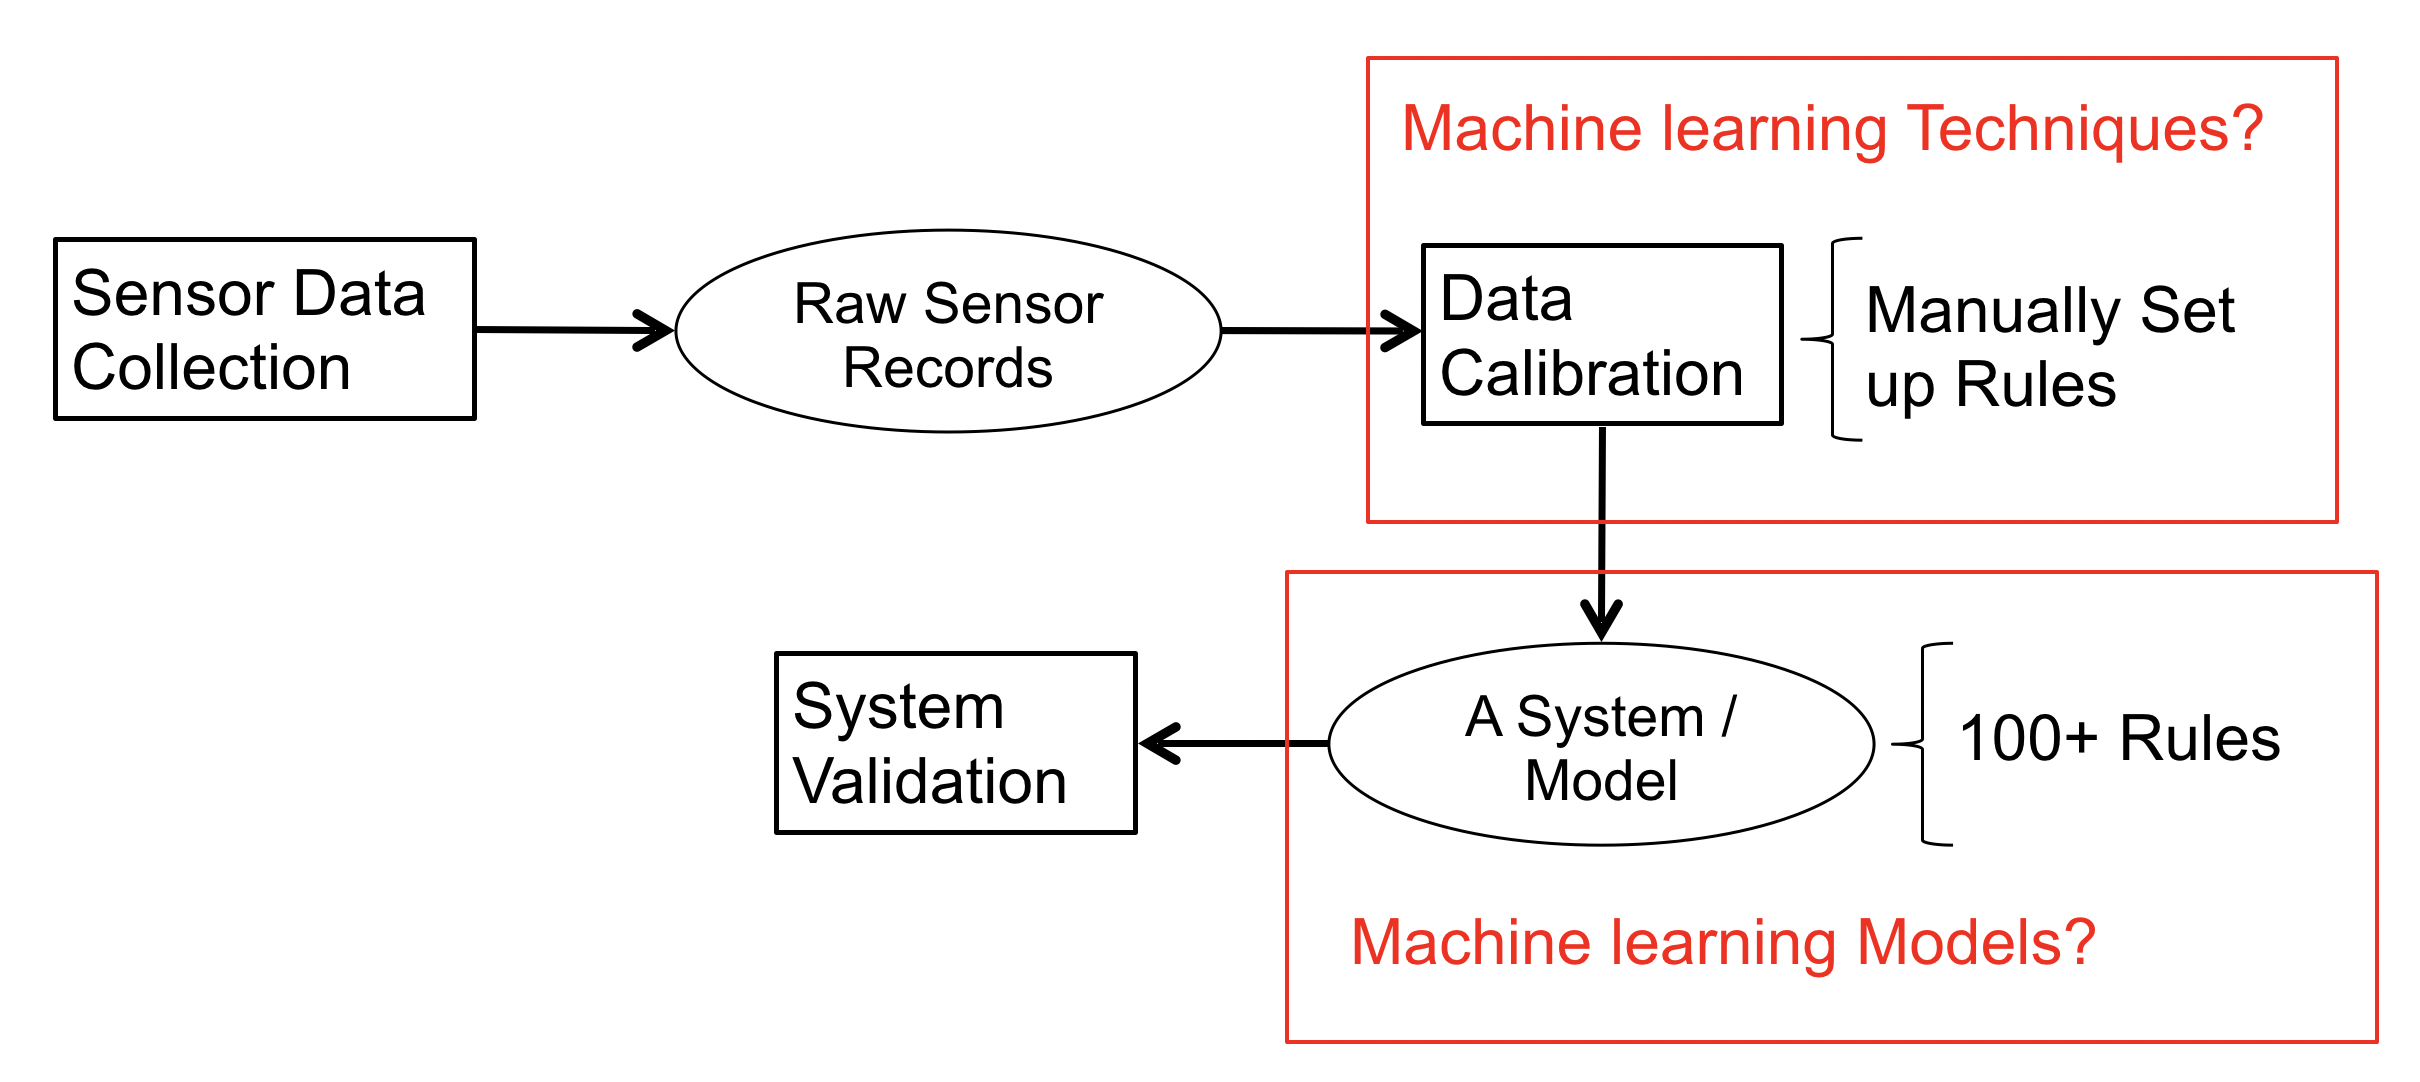
\includegraphics[width=0.75\textwidth]{related_work.png}
	\caption{The-State-of-the-Art Strategy of Blip Systems A/S}
	\label{fig:strategy_of_blip}
\end{figure}

\par
This project focuses on exploring machine learning techniques to distinguish and classify the raw sensor data of mobile devices. We should provide a more efficient solution for data calibration and modelling without the need for fine-grained manually created logic. Rather than analysing the data of the entire airport, a specific area - the arrival gate - was chosen.\newline

\par
The involved data set is a set of measurements collected from the sensors placed throughout the area. The raw, multidimensional data comes with intricacies of wireless signals and mobile device, such as variance in signal strength or edge cases create by different device usage patterns. This poses a significant challenge for data processing, which is why the data will need to be modelled to both represent the behaviour of passengers appropriately, as well as conform to the constraints of machine learning techniques to be utilised. \newline

\par
To achieve the goal of this project, the following methods will be used:

We will conduct our initial experiments using Label propagation as a baseline method with the focus on modelling the similarities among data in form of multivariate times series. The baseline will serve us as a simple method to get some initial results and help us to better understand the data, as well as to decide on further direction.
Afterwards, we will experiment with Decision Trees, a feature-centric technique, which will demand features to be extracted from the data (feature engineering).
Finally, the last stage will require a more complex, deep learning model such as Convolutional Neural Networks, where the objective will be to discover and learn patterns in the data automatically.
\chapter{Related Work}
\label{chap:RelWork}
\section{Overview}
\par
In general, machine learning tasks can be divided into supervised and unsupervised learning. In supervised learning, new data can be analysed based on previous experience, while unsupervised learning does not rely on prior information about labels for its processes. Given the scenario described, classification of a passenger is variable dependent on other provided information, we can safely state that we are facing a supervised learning task.\\

\par
Furthermore, supervised learning covers two classes of problems - classification and regression. When classifying, the task is to identify a group in which a new observation should belong. On the other hand, regression aims to determine a value on a continuous scale from given data. 

\section{Classification}
Since this project is concerned with categorising mobile devices (passengers/individuals) into different classes, our activities and experiments will naturally fall under classification. 

\par
For an overview of classification, the following is a short description of a few commonly used methods.

\subsection{\texorpdfstring{$k$NN}{kNN}}
The $k$-nearest-neighbours algorithm ($k$NN) is an intuitive machine learning method used for both classification and regression in multidimensional feature space. The label of the data to be classified is propagated from its $k$ nearest labelled data points. This depends on the chosen distance measure.\\

\par
More precisely, given a distance measure, the distances between every pair of points are calculated. When a new point is observed, it is assigned a label according to the majority of votes of the $k$ nearest points, where $k$ is a user-defined constant. Note that a larger $k$ generally reduces the effect of noise, but yields less distinct label groups.\\

\subsection{Perceptron}
The perceptron is a linear classifier used to determine a (binary) class of a vector. A Perceptron calculates the inner product of its $n$ weights and the $n$ dimensional input vector, adds a weighted bias to adjust the $y$ intercept of the linear separation line, and puts the result into a transfer function, ensuring that the result is binary. The weights are usually initialised as small random values and are iteratively adjusted during training to linearly separate the two classes.

\subsection{Naive Bayes}
Naive Bayes is a probabilistic classifier based on Bayes' theorem. The probabilities of each class are derived from the training data features usually using the maximum likelihood method, assuming independence between features. To classify unobserved data, probabilities of each class given input data features are calculated, and the most probable class is selected as the label.

\subsection{Recurrent neural network}
Recurrent neural network is a class of artificial neural networks that, in contrary to feed-forward neural networks, takes in account the internal state of a neuron, making it more suitable for time series processing.\\

\par
A fully recurrent neural network contains multiple layers of neurons, where each neuron is connected to every neuron of the successive layer, where each connection has a real-valued weight. The input layer consists of $n$ neurons, where $n$ is the number of features of the data. Training consists of presenting the selected $m \times n$ data to the network, where $n$ is the number of features and $m$ is the length of sequences, and its label. Throughout the training process, weights are adjusted to reflect the class separation. When unobserved data are presented, the correct label is determined from the previously calculated weights.


%\begin{example}
%	To obtain a better understanding of the $k$NN algorithm, consider the following dataset.
%	\begin{figure}[H]
%		\centering
%		\begin{tabular}{|c|c|}\hline
%			\textbf{Point} & \textbf{Label} \\ \hline
%			$(4,5)$ & 1 \\
%			$(3,4)$ & 1 \\
%			$(2,1)$ & 0 \\
%			$(3,3)$ & 0 \\
%			$(1,2)$ & 0 \\
%			$(4,3)$ & ? \\ \hline
%		\end{tabular}
%	\end{figure}
%	
%	In order to determine the label of $(4,3)$, it is required to calculate its distances to the labelled points. Using Euclidean distance measure, we obtain the following values.
%	
%	\begin{figure}[H]
%		\centering
%		\begin{tabular}{|c|c|}\hline
%			\textbf{Point} & \textbf{Distance} \\ \hline
%			$(4,5)$ & $2$ \\
%			$(3,4)$ & $\sqrt{2}$ \\
%			$(2,1)$ & $2\sqrt{2}$ \\
%			$(3,3)$ & $1$ \\
%			$(3,2)$ & $\sqrt{10}$ \\ \hline
%		\end{tabular}
%	\end{figure}
%	
%	Predicted labels can differ by the choice of $k$ to be used. Low values tend to lead to over-fitting while big values tend to lead to under-fitting. For the sake of demonstration, we will use $3$NN without deeper analysis of the data. The point $(4,3)$ will be then assigned a label based on labels of his three nearest neighbours, which are the points $(3,3)$, $(3,4)$ and $(4,5)$, carrying labels 0, 1 and 1. The label of $(4,3)$ will therefore be predicted to be 1.
%\end{example}
\bigskip
A similar task has already been handled in \cite{PredictingUserMovements} where authors use Recurrent Neural Network to predict the movement of an individual, reaching up to 90\% prediction accuracy. Note that the dataset used for this experiment was created for the sole purpose of testing the used method. Therefore the recorded measurements are not as sparse as in a real-life scenario and allow much more effective learning.\\

\par
Aside from RNNs, Convolutional Neural Networks have also been exploited for multivariate time series classification \cite{CNNTimeSeriesPred, Yang2015DeepCN}, offering us multiple approaches to our problem.\\


\chapter{Preliminaries}\label{chap:Prelimi}
\section{Time series}
\label{sec:time_series}
The airport data we will be working with consists of readings from multiple sensors strategically located throughout a selected region of the airport. Therefore, in order to model a single individual in the raw data, we will use multivariate time series. \\

In our case, a passenger is the same as a mobile device, and a mobile device is characterised by its address. We will therefore use the terms "passenger", "mobile device" and "mobile address" interchangeably. \\


We define our sensor time series as

\begin{align*}
	X_{i,j} = \langle (t_1, c_1), (t_2, c_2), \cdots, (t_n, c_n)\rangle,
\end{align*}

where

\begin{itemize}
	\item $i$ is the index of the mobile address
	\item $j$ is the index of the sensor
	\item $n$ is the count of measurements of the $i$-th mobile device taken by the $j$-th sensor
	\item $c_k$ is the signal strength at time $t_k$, where $1 \leq k \leq n$
\end{itemize}

Since each mobile device is recorded by multiple sensors, we need to model each mobile device as a multivariate time series, which we define as:

\begin{align*}
	\mathcal{X}_i = (X_{i,1}, X_{i,2}, \cdots, X_{i,m})
\end{align*}

\pagebreak

where

\begin{itemize}
	\item $i$ is the index of the mobile device
	\item $X_{i,1}, \cdots, X_{i,m}$ are the sensor time-series for the $i$-th device
	\item $m$ is the number of sensors
\end{itemize}

\section{Problem definition}

The project objective is to find a model that includes and describes all the information about a passenger and use it together with machine learning techniques to assign a passenger to a class label.\\
The existing data were modelled in \cref{sec:time_series} in terms of multivariate time series:
\begin{align*}
	\mathcal{X}_i = (X_{i,1}, X_{i,2}, \cdots, X_{i,m})
\end{align*}

Now, the set of labels $l = \{\text{manual},\ \text{staff},\ \text{no-q},\ \text{privium}\}$ can be introduced, where

\begin{itemize}
	\item \textit{manual} is a standard passenger
	\item \textit{staff} is a member of the airport staff
	\item \textit{no-q} is a passenger that can use electronic passport control
	\item \textit{privium} is a passenger with priority pass
\end{itemize}

Further, L = $\{(\mathcal{X}_1, l_1),(\mathcal{X}_2, l_2), \cdots, (\mathcal{X}_n, l_n)\}$ defines a set of passengers with the corresponding labels $\{l_1, l_2, \cdots, l_n \} \in l$.\\


Given a set of passengers $\{(\mathcal{X}_{n+1}, l_{n+1}), \cdots, (\mathcal{X}_{n+m},l_{n+m}) \}$ with unobserved labels $\{l_{n+1}, \cdots, l_{n+m} \}$, the aim is to assign one of the defined labels from $l$ to each label from unobserved labels set. 

\chapter{Data analysis}
\section{General statistics}
\label{sec:general_statistics}
The data we are working with represents sensor readings over a total of 7 days of airport activity, set in September 2018. \\
The data was filtered beforehand to contain only the measurements that correspond to Bluetooth addresses that are already labelled. These correspond to 7.612.286 readings which we filtered further down to 974.152 measurements, only the ones recorded within the arrival area. Therefore we are left to work with 13.530 unique mobile devices. The labels for those addresses are the following (also seen visualised in \cref{fig:stats_labels}):

\begin{itemize}
	\item 8.045 Staff
	\item 3.574 Manual
	\item 1.633 No-q
	\item 278 Privium
\end{itemize}

\begin{figure}[H]
    \centering
    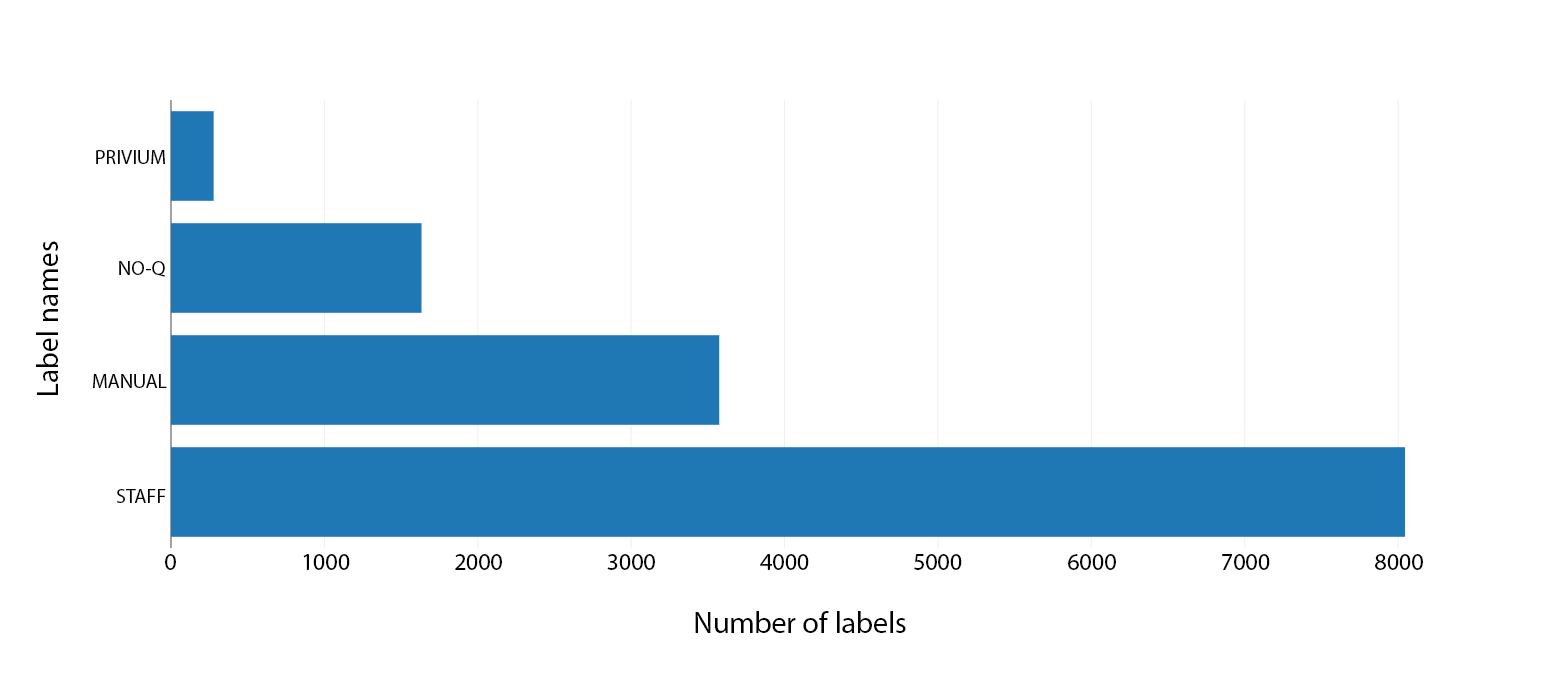
\includegraphics[width=.75\textwidth]{Pictures/Labels.png}
    \caption{Labels}
    \label{fig:stats_labels}
\end{figure}

The value of the signal strength measurements vary between -75 and -3. The value -73 is the most common signal strength, representing 15.34\% of the total measurements. The overall average signal strength is -66.34. This may be seen in \cref{fig:sensor_strength_readings}.\\

\begin{figure}[H]
    \centering
    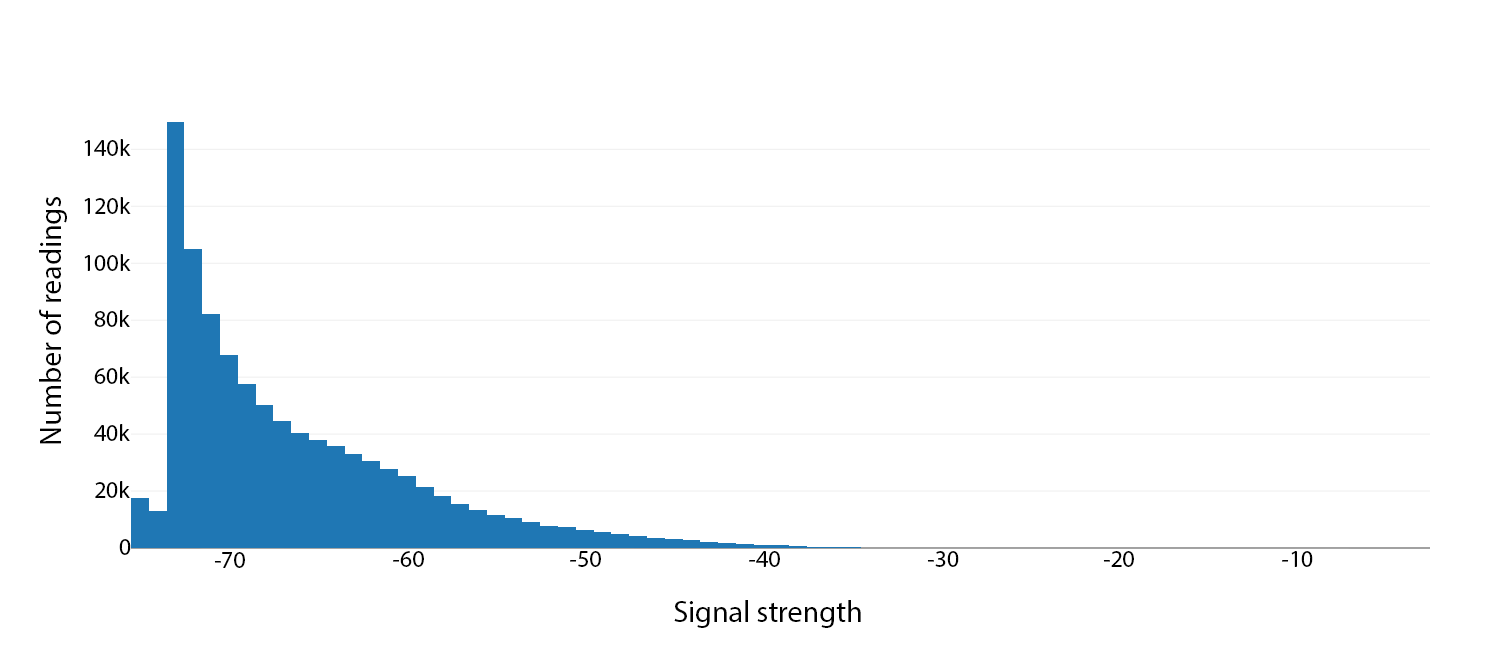
\includegraphics[width=.8\textwidth]{Pictures/Sensor_Strength_Readings.png}
    \caption{Sensor strength readings}
    \label{fig:sensor_strength_readings}
\end{figure}

The chart in \cref{fig:stat:readingspersensor} shows the amount of readings that are taken of members of each class by the different sensors present. The sensor with the most readings is P2 which recorded 88.896 signals. While other nearby sensors have close to that amount of readings, the lowest amount of measurements is from the QE1 sensor that recorded 32.802 signals.\\

\begin{figure}[H]
    \centering
    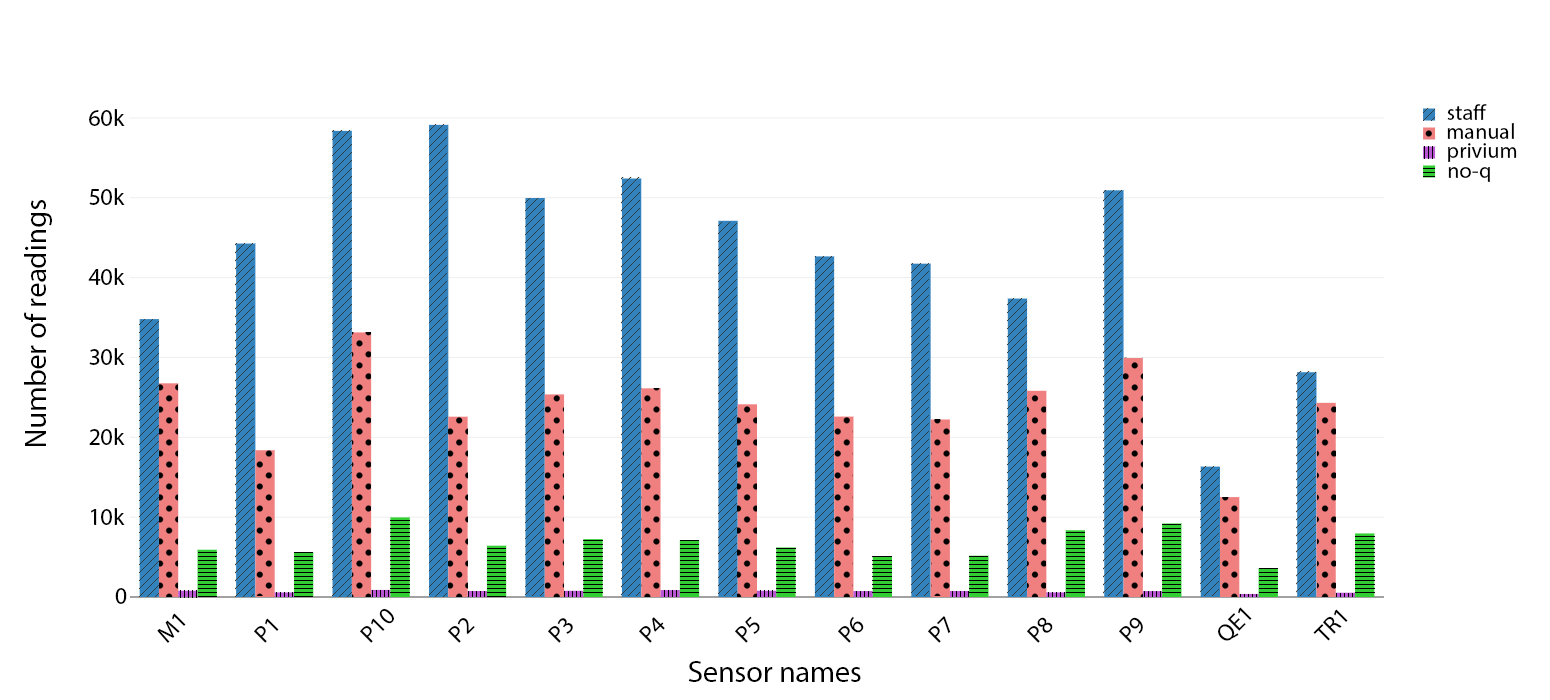
\includegraphics[width=.8\textwidth]{Pictures/Readings_per_sensor.png}
    \caption{Readings per sensor}
    \label{fig:stat:readingspersensor}
\end{figure}

\pagebreak

The distribution in \cref{fig:stat:timespentdistbylabel} displays the amounts of time (in minutes) spent in the area by members of each of the four label groups. We observe that, regardless of label, the majority is in and out in less than 45 minutes.

\begin{figure}[H]
    \centering
    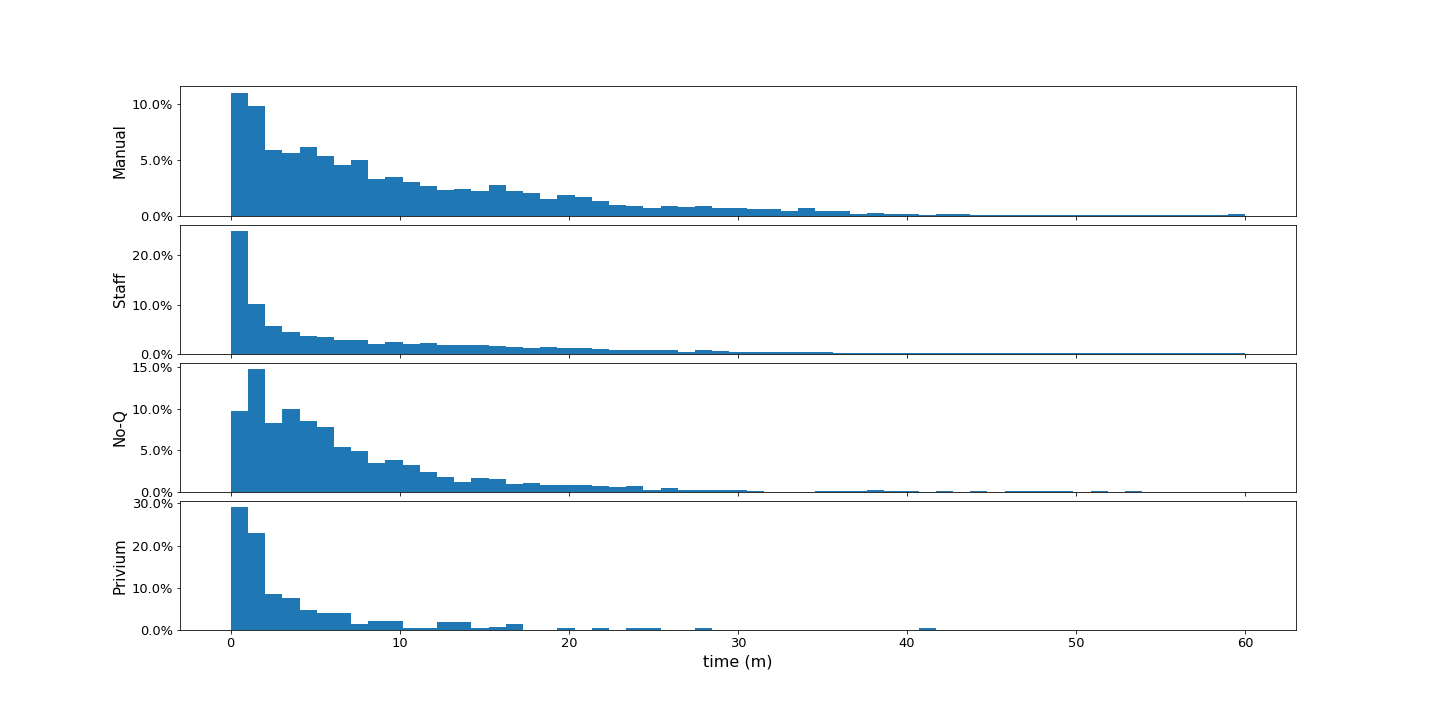
\includegraphics[width=1\textwidth]{Pictures/timespentdistbylabel.png}
    \caption{Distribution of time spent in the area, by label}
    \label{fig:stat:timespentdistbylabel}
\end{figure}

The following percentages represent the ratio of devices in each group that pass through in less than 45 minutes:

\begin{itemize}
	\item Manual:   96.1\%
	\item Staff:    88.9\%
	\item No-Q:     97.6\%
	\item Privium:  95.7\%
\end{itemize}

For example, 96.1\% of addresses labelled as "Manual" take less than 45 minutes to pass.

\chapter{Modelling the data}\label{chap:datamodelling}

This chapter focuses on modelling each address as a multidimensional time series that we can then work with. The general idea is to form a table with every sensor time series representing a column. We will then fill the table with values and interpolate the missing ones.

Recall that we have previously defined the time series for each Bluetooth address $i$ and sensor $j$ as

\begin{align*}
	X_{i,j} = \langle (t_1, c_1), (t_2, c_2), \cdots, (t_n, c_n)\rangle
\end{align*}

where

\begin{itemize}
	\item $i$ is the index of the mobile device
	\item $j$ is the index of the sensor
	\item $n$ is the count of measurements of the $i$-th mobile device taken by the $j$-th sensor
	\item $c_k$ is the signal strength at time $t_k$, where $0 \leq k \leq n, k \in \mathbb{N}$
\end{itemize}

Starting from this, we merge on the sensors, obtaining

\begin{align*}
	\mathcal{X}_i = \langle (t_1, c_1, s_1), (t_2, c_2, s_2), \cdots, (t_m, c_m, s_m)\rangle
\end{align*}

where  

\begin{itemize}
	\item $i$ is the index of the mobile device
	\item $m$ is the number of all measurements taken by all sensors on the $i$-th mobile device
	\item $c_k$ is the signal strength at time $t_k$, where $0 \leq k \leq m, k \in \mathbb{N}$
	\item $s_k$ is a sensor
	\item events ordered by time: $0 \leq i < j \leq m \implies t_i < t_j, \forall i, j \in \mathbb{N}$
\end{itemize}

so that each $(t,c,s)$ pair represents the strength $c$ of the measurement taken by sensor $s$ at time $t$ of the Bluetooth address $\mathcal{X}_i$.\\

\par
We first apply the following transformation, which makes $t_0$ 0 and keeps the relative distances to the other measurement time-stamps:
\begin{align*}
	t_k := t_k-t_0, \forall k \in [0,m]
\end{align*}

The result is an array that might look like
\begin{align*}
    [(0,-80,S1), (3,-60,S1), (3,-70,S2), (5,-60,S3), \\
    (6,-30,S1), (7,-30,S2), (9,-80,S1), (10,-70,S3)]
\end{align*}

We can now define an empty table T of size $|S| \times t_m$ ($t_m = \max (t_1...t_m$)), and fill it out as follows:
\begin{align*}
    T_{s_kt_k} := c_k, \forall (t_k, c_k, s_k) \in \mathcal{X}_i
\end{align*}

This results in \cref{fig:datamodelling:tables:1}:

\begin{figure}[H]
    \label{fig:datamodelling:tables}
    \centering
    \begin{minipage}[t]{0.3\textwidth}
        \centering
        \begin{tabular}{ |c||c|c|c| }
             \hline
             t & S1 & S2 & S3 \\
             \hline
             0  & -70 &  & \\ 
             1  &  &  & \\ 
             2  &  &  & \\ 
             3  & -60 & -70 & \\ 
             4  &  &  & \\ 
             5  &  &  & -60 \\ 
             6  & -30 &  & \\ 
             7  &  & -30 & \\ 
             8  &  &  & \\ 
             9  & -73 &  & \\ 
             10 &  &  & -70 \\
             \hline
        \end{tabular}
        % just edit the three \subcaption
        % also you can use \subcaption instead of \subcaption* if you want them to be labelled (a, b, c by default), this can for sure be changed
        \subcaption{Step 1}
        \label{fig:datamodelling:tables:1}
    \end{minipage}
    \hfill
    \begin{minipage}[t]{0.3\textwidth}
        \centering
        \begin{tabular}{ |c||c|c|c| } 
             \hline
             t & S1 & S2 & S3 \\
             \hline
             0  & -70 & -75 & -75 \\ 
             1  &  &  & \\ 
             2  &  &  & \\ 
             3  & -60 & -70 & \\ 
             4  &  &  & \\ 
             5  &  &  & -60 \\ 
             6  & -30 &  & \\ 
             7  &  & -30 & \\ 
             8  &  &  & \\ 
             9  & -70 &  & \\ 
             10 & -75 & -75 & -70 \\
             \hline
        \end{tabular}
        \subcaption{Step 2}
        \label{fig:datamodelling:tables:2}
    \end{minipage}
    \hfill
    \begin{minipage}[t]{0.3\textwidth}
        \centering
        \begin{tabular}{ |c||c|c|c| } 
             \hline
             t & S1 & S2 & S3 \\
             \hline
             0  & -70 & -75 & -75 \\ 
             1  & -66 & -73 & -72 \\ 
             2  & -63 & -72 & -69 \\ 
             3  & -60 & -70 & -66 \\ 
             4  & -50 & -60 & -63 \\ 
             5  & -40 & -50 & -60 \\ 
             6  & -30 & -40 & -62 \\ 
             7  & -43 & -30 & -64 \\ 
             8  & -66 & -45 & -66 \\ 
             9  & -70 & -60 & -68 \\ 
             10 & -75 & -75 & -70 \\
             \hline
        \end{tabular}
        \subcaption{Step 3}
        \label{fig:datamodelling:tables:3}
    \end{minipage}
    % main caption isnt mandatory of course
    \caption{Construction of the table for modelling multi-dimensional time-series of a mobile device}
\end{figure}



If any of the sensors' values at time 0 or $k_m$ are undefined, we define them as -75, the minimum signal strength, as illustrated in \cref{fig:datamodelling:tables:2}. We can finally interpolate the missing data.\\

\par
The idea is, for each sensor's time series $s_k \in S$, for each index that does not have a reading, we find the previous and next index in the time series for which we have values: $(p_i, p), (n_i, n),\ p_i<i<n_i$. We are guaranteed to have a previous and next reading thanks to (b). Using basic algebra we can then define and calculate $\alpha$ and $\beta$ for a linear function $f(x)=\alpha x+\beta$ so that $f(p_i)=p$ and $f(n_i)=n$. We then simply assign

\begin{align*}
     T_{s_k t_i} := f(i)
\end{align*}

We are thus left with the table in \cref{fig:datamodelling:tables:3}.

\chapter{Baseline - Label Propagation}\label{chap:base}
\section{Label Propagation}
\label{sec:label_prop}
\par
Label propagation is a semi-supervised machine learning algorithm during which a node's label is propagated to its neighbours according to their proximity. The labelled data serve as sources to iteratively propagate labels through unlabelled data, allowing data that are not direct neighbours of labelled points to be labelled based on their unlabelled neighbours.\\

\subsection{Data Pre-processing}
\par
The input data are expected by the label propagation algorithm in a specific format and therefore our data have to be processed as follows before the actual algorithm starts.\\

\par
Let $(\mathcal{X}_1, l_1), \cdots, (\mathcal{X}_\ell, \cdots, l_\ell)$ be the labelled data and $(\mathcal{X}_{\ell+1}, l_{\ell+1}),\cdots,(\mathcal{X}_{\ell+u}, l_{\ell+u})$ the unlabelled data, i.e. $Y_U = \{l_{\ell+1}, \cdots l_{\ell+u} \}$ are unobserved. To estimate the labels of $Y_U$ from $\mathcal{X} = \{ \mathcal{X}_1,\cdots, \mathcal{X}_\ell, \mathcal{X}_{\ell+1},\cdots, \mathcal{X}_{\ell+u} \}$ and $Y_L = \{ l_1,\cdots, l_{\ell} \}$, we create a fully connected graph with nodes representing individual passenger's multivariate time series. We represent this graph by the adjacency matrix $W$, where the weight of the edge between nodes $i$ and $j$ is calculated as the similarity of time series $\mathcal{X}_i$ and $\mathcal{X}_j$, as described in \ref{similarity_computation}. Hence

\begin{align*}
    W_{ij} = sim(\mathcal{X}_i, \mathcal{X}_j)
\end{align*}

\par
Finally, we define a $(\ell+u)\times L$ label matrix $Y_0$, where $L$ represents the number of labels in our data set. $Y_{0_{il}}$ represents the probability of $i$-th data point holding the $l$-th label.\\


\subsection{The Algorithm}
\par
Once the input matrices has been prepared, the algorithm executes the following steps:
\begin{enumerate}
    \item Convert the adjacency matrix $W$ into a probabilistic transition matrix $T$, where $T_{ij}$ represents the probability of $i$ adopting the label of $j$:
    \begin{align*}
        T_{ij} = P(j \xrightarrow{} i) = \frac{W_{ij}}{\sum_{k=1}^{\ell+u}W_{kj}}
    \end{align*}
    
    \item Update the label probabilities by propagating 
    \begin{align*}
        Y_{t+1} = T\times Y_t;\quad t = \{0,1,2\cdots,n\}
    \end{align*}
    \item Row-normalise $Y_{t+1}$ to maintain the probability distribution representation:
    \begin{align*}
        Y_{{(t+1)}_{il}} = \frac{Y_{{(t+1)}_{il}}}{\sum_{k=1}^{L}Y_{{(t+1)}_{ik}}}
    \end{align*}
    \item Clamp observed data. Repeat from step 2 until $Y$ converges.
\end{enumerate}

During step 1, nodes propagate their labels based on the probabilities, resulting in the updated label matrix $Y_{t+1}$. During step 2, the rows of $Y_{t+1}$ are normalised to represent a probability distribution. In step 3, the labelled data points in $Y_{t+1}$ are set to their initial values to maintain their persistence and help unlabelled data during learning.

\par
After the iterative procedure terminates, the label matrix $Y_n$ is obtained from where the label with highest probability is used as the estimated label. Note that although the termination time $n$ is unknown, it is guaranteed that it converges in a finite number of iterations.\\

\begin{example}
    As an example, consider the following multivariate time series $\mathcal{X}_i$ with data \newline $\langle (t_1, c_1), \cdots, (t_n, c_n)\rangle$ on sensors $(X_{i,1}, \cdots, X_{i,m})$ and with labels $l_i$:
    
    \begin{figure}[H]
        \centering
        \begin{tabular}{|c|c|c|c|}
            \hline
             Time series & Sensor & Data & Label \\ \hline
             \multirow{3}{*}{$\mathcal{X}_1$} & $X_{1,1}$ & $\langle (0, 10), (1, 15), (2, 10)\rangle$ & \multirow{3}{*}{0} \\
                                              & $X_{1,2}$ & $\langle (0, 20), (1, 25), (2, 15)\rangle$ & \\
                                              & $X_{1,3}$ & $\langle (0, 20), (1, 15), (2, 20)\rangle$ & \\ \hline
             \multirow{3}{*}{$\mathcal{X}_2$} & $X_{2,1}$ & $\langle (0, 5), (1, 20), (2, 15)\rangle$ & \multirow{3}{*}{0} \\
                                              & $X_{2,2}$ & $\langle (0, 10), (1, 25), (2, 5)\rangle$ & \\
                                              & $X_{2,3}$ & $\langle (0, 15), (1, 5), (2, 10)\rangle$ & \\ \hline
             \multirow{3}{*}{$\mathcal{X}_3$} & $X_{3,1}$ & $\langle (0, 25), (1, 30), (2, 30)\rangle$ & \multirow{3}{*}{1} \\
                                              & $X_{3,2}$ & $\langle (0, 20), (1, 20), (2, 20)\rangle$ & \\
                                              & $X_{3,3}$ & $\langle (0, 10), (1, 5), (2, 10)\rangle$ & \\ \hline
             \multirow{3}{*}{$\mathcal{X}_4$} & $X_{4,1}$ & $\langle (0, 20), (1, 25), (2, 40)\rangle$ & \multirow{3}{*}{1} \\
                                              & $X_{4,2}$ & $\langle (0, 25), (1, 10), (2, 10)\rangle$ & \\
                                              & $X_{4,3}$ & $\langle (0, 15), (1, 45), (2, 25)\rangle$ & \\ \hline
             \multirow{3}{*}{$\mathcal{X}_5$} & $X_{5,1}$ & $\langle (0, 5), (1, 5), (2, 10)\rangle$ & \multirow{3}{*}{?} \\
                                              & $X_{5,2}$ & $\langle (0, 10), (1, 15), (2, 5)\rangle$ & \\
                                              & $X_{5,3}$ & $\langle (0, 25), (1, 20), (2, 35)\rangle$ & \\ \hline
        \end{tabular}
    \end{figure}
    
    Firstly, we construct the similarity matrix $W$ which represents the fully connected graph of passengers.
    
    Given that weight between nodes $i$ and $j$ is calculated as $w_{ij} = sim(X_i, X_j)$, we obtain:
    \begin{align*}
        W = 
        \begin{bmatrix}
            1    & 0.95 & 0.25 & 0.15 & 0.80 \\
            0.95 & 1    & 0.30 & 0.25 & 0.85 \\
            0.25 & 0.30 & 1    & 0.95 & 0.20 \\
            0.15 & 0.25 & 0.95 & 1    & 0.10 \\
            0.80 & 0.85 & 0.20 & 0.10 & 1
        \end{bmatrix}
    \end{align*}
    
    To transform $W$ into probabilistic transition matrix $T$, we row-normalise the matrix:
    \begin{align*}
        T_{ij} = \frac{W_{ij}}{\sum_{k=1}^{5}W_{kj}}
    \end{align*}
    
    Therefore, the probabilistic transition matrix $T$ looks as follows.
    \begin{align*}
        T = 
        \begin{bmatrix}
            0.317 & 0.283 & 0.094 & 0.061 & 0.271 \\
            0.302 & 0.299 & 0.111 & 0.102 & 0.288 \\
            0.079 & 0.089 & 0.370 & 0.388 & 0.068 \\
            0.048 & 0.075 & 0.352 & 0.408 & 0.034 \\
            0.254 & 0.254 & 0.074 & 0.041 & 0.339
        \end{bmatrix}
    \end{align*}
    
    Construction of label matrix $Y$ is straightforward. Note that unobserved data can be initialised with any probability.
    
    \begin{align*}
        Y_0 = 
        \begin{bmatrix}
            1   & 0 \\
            1   & 0 \\
            0   & 1 \\
            0   & 1 \\
            0.5 & 0.5 
        \end{bmatrix}
    \end{align*}
    
    Finally, the iterative algorithm can start. In the first step, we propagate $Y \xleftarrow{} TY$:
    
    \begin{align*}
        Y_1 =
        \begin{bmatrix}
            0.317 & 0.283 & 0.094 & 0.061 & 0.271 \\
            0.302 & 0.299 & 0.111 & 0.102 & 0.288 \\
            0.079 & 0.089 & 0.370 & 0.388 & 0.068 \\
            0.048 & 0.075 & 0.352 & 0.408 & 0.034 \\
            0.254 & 0.254 & 0.074 & 0.041 & 0.339
        \end{bmatrix}
        \times
        \begin{bmatrix}
            1   & 0 \\
            1   & 0 \\
            0   & 1 \\
            0   & 1 \\
            0.5 & 0.5 
        \end{bmatrix}
        = 
        \begin{bmatrix}
            0.7355 & 0.2905 \\
            0.7450 & 0.3570 \\
            0.2020 & 0.7920 \\
            0.1400 & 0.7770 \\
            0.6775 & 0.2845
        \end{bmatrix}
    \end{align*}
    
    In step two, we have to row-normalise the newly obtained $Y$:
    \begin{align*}
        Y_1 =
        \begin{bmatrix}
            0.7168 & 0.2832 \\
            0.6760 & 0.3240 \\
            0.2032 & 0.7968 \\
            0.1527 & 0.8473 \\
            0.7042 & 0.2958
        \end{bmatrix}
    \end{align*}
    
    And finally, we clamp the labelled data to their original values, obtaining
    \begin{align*}
        Y_1 =
        \begin{bmatrix}
            1      & 0      \\
            1      & 0      \\
            0      & 1      \\
            0      & 1      \\
            0.7042 & 0.2958
        \end{bmatrix}
    \end{align*}
    
    This procedure is repeated until the values of $Y_n$ converge, giving us the result
    \begin{align*}
        Y_n =
        \begin{bmatrix}
            1      & 0      \\
            1      & 0      \\
            0      & 1      \\
            0      & 1      \\
            0.8154 & 0.1846
        \end{bmatrix}
    \end{align*}
    
    Therefore, the time series $\mathcal{X}_5$ is predicted to carry label $1$ with probability $0.8154$ and label $0$ with probability $0.1846$.
\end{example}

\section{Similarity computation}
\label{similarity_computation}
\par
In order to be able to transform our data to the input graph form required for label propagation, we first need to introduce a similarity function.
\par
\medskip
Given the multidimensional time-series for two mobile devices, $\mathcal{X}_a$ and $\mathcal{X}_b$, we can build the tables $T_a$ and $T_b$, using the procedure defined in \cref{chap:datamodelling}, with each table being initialised with the shape $m \times n$, where $m$ is the number of sensors and $n$ is the overall latest time stamp from $\mathcal{X}_a$ or $\mathcal{X}_b$. The similarity function $sim$ should then compare $T_a$ and $T_b$, resulting in a similarity measure $sim(T_a,T_b)$ in the interval [0,1].
\par
\medskip
\par
First, we need to calculate the overall distance between $T_a$ and $T_b$. The data for each mobile device consists of a set of time-series, each corresponding to the data for one sensor, represented as a column in the table. Based on that we can calculate a distance for every sensor (column) in the table as the sum of cell-by-cell differences. These sensor distances can be summed further, resulting in a single distance value between $T_a$ and $T_b$.\\

\par
Overall, we can define this calculation for tables $T_a$ and $T_b$, both of shape $n \times m$ as the following absolute-valued matrix difference of table values:
\begin{equation*}
    dist(T_a,T_b) = \sum_{i=1}^n \sum_{j=1}^m |{T_a}_{i,j} - {T_b}_{i,j}|
\end{equation*}
where
\begin{itemize}
    \item $n$ is the number of rows in tables $T_a$, $T_b$
    \item $m$ is the number of columns in tables $T_a$, $T_b$
    \item ${T_a}_{i,j}$ is the value in the $i$-th row and $j$-th column of $T_a$
    \item ${T_b}_{i,j}$ is the value in the $i$-th row and $j$-th column of $T_b$
\end{itemize}

\par
Now, in order to transform the absolute distance into a similarity measure in the interval [0,1], we can normalise the distance using the maximum possible distance between two tables:
\begin{equation*}
    sim(T_a,T_b) = \frac{dist_{max} - dist(T_a,T_b)}{dist_{max}}
\end{equation*}
where $dist_{max}$ can be calculated as:
\begin{equation*}
    dist_{max} = n \cdot m \cdot v_{max}
\end{equation*}
where $v_{max}$ is the maximum absolute value of a cell in a table of shape $n \times m$.\\

\par
To illustrate this, we can use the table in \cref{fig:datamodelling:tables:3} on page \pageref{fig:datamodelling:tables:3}. We know that the absolute value of a cell will never be higher than 75, therefore we let $v_{max}$ be 75. As the table contains 3 columns (sensors) and 10 rows (time), we calculate $dist_{max}$ as $n \cdot m \cdot v_{max} = 10 \cdot 3 \cdot 75 = 2250$. 

\par
The intuition behind using $dist_{max}$ is to define the global hypothetical maximum for any similarity computation in our data, given the shape of the pre-processed mobile address table models. The $dist_{max}$ then serves as a common constant, with distances being normalised into a similarity interval of [0,1], relative to this constant.

\par
An overview of the similarities calculated using $sim(T_a,T_b)$ on our data may be seen in \cref{fig:results:similarity_distribution} of the results section of the report.


\section{Results}
In order to test label propagation on our data, we have applied the similarity computation formulated in the previous section to calculate the similarities for a portion of our data set.\par
\medskip
We have selected 275 mobile addresses per class, representing the total of 1100 nodes in the input graph for label propagation. The similarity computation was then performed on each of the 604450 edges in the graph (each pair of mobile addresses) to obtain the adjacency matrix $W_{ij}$. The distribution of similarity scores between all the compared pairs of addresses may be seen in Figure \ref{fig:results:similarity_distribution}. \par

\begin{figure}[H]
    \centering
    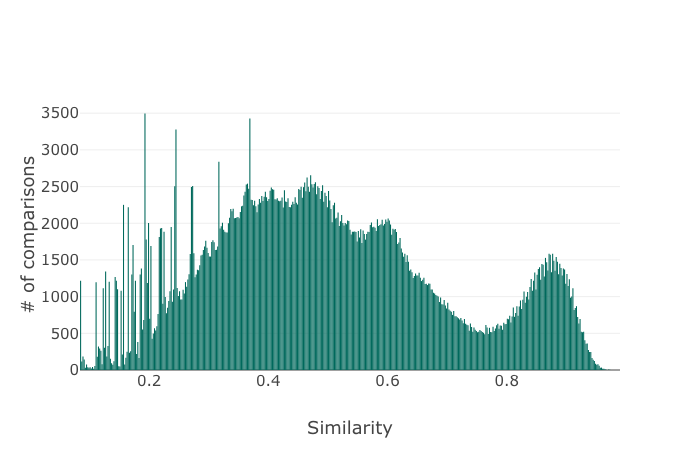
\includegraphics[width=.7\textwidth]{Pictures/similarity_distribution_plot.png}
    \caption{Distribution of similarity scores calculated from all pairs of 1100 addresses, using the similarity computation $sim(T_a,T_b)$ from Section \ref{similarity_computation}}
    \label{fig:results:similarity_distribution}
\end{figure}

\medskip
For training data (seeds), we have selected 90 addresses for each class (360 addresses in total, corresponding to roughly 1/3 of unique addresses in the input graph), for which we have defined ground truth labels $Y_L$.\par
\medskip

Given this configuration, running the model on the test data resulted in an overall accuracy of 36\%, and per-label accuracies of 37\%, 3\%, 67\% and 40\% for "manual", "staff", "no-q" and "privium" respectively. A more detailed breakdown of how the model predicted different examples in test data may be seen in the confusion matrix below.

\begin{figure}[H]
    \centering
    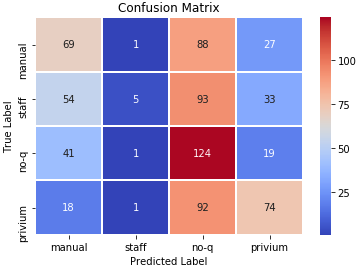
\includegraphics[width=.5\textwidth]{Pictures/label_prop_confusion.png}
    \caption{Label propagation results (confusion matrix)}
    \label{fig:label_prop:confusion_matrix}
\end{figure}
\pagebreak

\subsection{Performance metrics}
\label{section:performance_metrics}
\subsubsection{Confusion matrix}
The confusion matrix from Figure \ref{fig:label_prop:confusion_matrix} gives a representation of the relationship between the ground truth and the predicted labels for each example in the test data. The rows in the matrix represent the true labels, while the columns represent the predicted labels. Inherently, the diagonal of the matrix represents the numbers of correctly classified examples for each label. Similarly, the tile in the fourth row and first column of the confusion matrix gives the number of examples where the true label was "privium", but the classifier predicted "manual".

\subsubsection{True positive, False positive, False negative and True negative}
\label{sec:true_positives}
For each label, we can also define the following measures, based on the confusion matrix:
\begin{itemize}
    \item \textbf{True positives (TP)} are the examples for which the true label was also the predicted label. Considering the confusion matrix $CM$:
        \begin{equation*}
            TP_l = CM_{l,l}
        \end{equation*}
    where $CM_{ll}$ is the value in the $l$-th row and $l$-th column of $CM$.
    
    \item \textbf{False positives (FP)} for label $l$ are all the examples that are not $l$, but were classified as $l$. Given the confusion matrix $CM$:
        \begin{equation*}
            FP_l = \sum_k CM_{k,l} - CM_{l,l}
        \end{equation*}
    where $CM_{k,l}$ is the value in the $k$-th row, $l$-th column of $CM$ and $CM_{l,l}$ is the value in the $l$-th row, $l$-th column of $CM$.
    
    \item \textbf{False negatives (FN)} for label $l$ are the examples with true label $l$ that have not been classified as $l$. In terms of confusion matrix $CM$:
    \begin{equation*}
        FN_l = \sum_k CM_{l,k} - CM_{l,l}
    \end{equation*}
    where $CM_{l,k}$ is the value in the $l$-th row, $k$-th column of $CM$ and $CM_{l,l}$ is the value in the $l$-th row, $l$-th column of $CM$.
    
    \item \textbf{True negatives (TN)} with respect to label $l$ are those examples for which the true label is not $l$, nor have they been classified as $l$. Given confusion matrix $CM$:
    \begin{equation*}
        TN_l = \sum_j\sum_k CM_{j,k} \quad j,k \neq l
    \end{equation*}
\end{itemize}

An illustration of these concepts ($TP$, $FP$, $FN$ and $TN$) on a confusion matrix for a given label (\textit{manual}) may be seen in \cref{fig:manual_tp_fn_tn_etc_example} below. 

\begin{figure}[H]
    \centering
    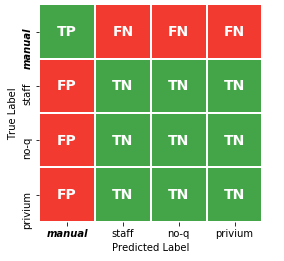
\includegraphics[width=.4\textwidth]{Pictures/manual_tp_fn_tn_example.png}
    \caption{$TP$, $FP$, $FN$ and $TN$ values illustrated on the confusion matrix for label \textit{manual}}
    \label{fig:manual_tp_fn_tn_etc_example}
\end{figure}

\subsubsection{Accuracy, recall and precision}
Given our true and predicted test data examples, we can calculate the (overall) \textbf{accuracy} simply as:
\begin{equation*}
    Accuracy = \frac{\text{Correctly Predicted Examples}}{\text{Total Examples}}
\end{equation*}
which can be calculated using the confusion matrix $CM$ as:
\begin{equation*}
    Accuracy = \frac{\sum\limits_{i=1}^{4} CM_{i,i}}{\sum\limits_{i=1}^{4}\sum\limits_{j=1}^{4} CM_{i,j}}
\end{equation*}
where $CM_{i,i}$ and $CM_{i,j}$ are the values of matrix $CM$ in the $i$-th row, $i$-th column and $i$-th row, $j$-th column respectively.\par
\medskip
\par
We will also define two concepts for measuring performance per-label: \textit{recall} and \textit{precision}.
\medskip
\par
\textbf{Recall} is the ratio of correctly predicted examples relative to all true examples of a given label in the test data, or mathematically, given the confusion matrix $CM$:  
\begin{equation*}
    Recall(l) = \frac{CM_{l,l}}{\sum\limits_{k=1}^{4} CM_{l,k}} = \frac{TP_l}{TP_l+FN_l}
\end{equation*}
where $l$ is number of a label with respect to rows and columns in the confusion matrix, $TP_l$ is the number of true positives and $FN_l$ the number of false negatives (\cref{sec:true_positives}).

\medskip
\par
\textbf{Precision} is the ratio of correctly predicted examples relative to the total of examples predicted for that label (correct and incorrect), or mathematically, given the confusion matrix $CM$:

\begin{equation*}
    Precision(l) = \frac{CM_{l,l}}{\sum\limits_{k=1}^{4} CM_{k,l}} = \frac{TP_l}{TP_l + FP_l}
\end{equation*}
where $l$ is number representation of a label with respect to rows and columns in the confusion matrix, $TP_l$ is the number of true positives and $FP_l$ is the number of false positives (\cref{sec:true_positives}). 

\subsection{Performance summary}
Having defined the performance measures, below is the performance summary for label propagation on our data, derived from the confusion matrix in Figure \ref{fig:label_prop:confusion_matrix}. 
\begin{table}[H]
    \centering 
    \begin{tabular}{c|c|c|c|}
        \cline{2-4}
                                                     & \textbf{Precision} & \textbf{Recall} & \textbf{Examples} \\ \hline
        \multicolumn{1}{|l|}{\textbf{manual}}        & 0.38               & 0.37            & 185               \\ \hline
        \multicolumn{1}{|l|}{\textbf{staff}}         & 0.62               & 0.03            & 185               \\ \hline
        \multicolumn{1}{|l|}{\textbf{no-q}}          & 0.31               & 0.67            & 185               \\ \hline
        \multicolumn{1}{|l|}{\textbf{privium}}       & 0.48               & 0.40            & 185               \\ 
        \hline \hline
        \multicolumn{1}{|l|}{\textbf{Average / Total}} & 0.45               & 0.37            & 740               \\ 
        \hline \hline
        \multicolumn{1}{|l|}{\textbf{Accuracy}}      & \multicolumn{3}{c|}{0.36}                                \\ \hline
    \end{tabular}   
    \caption{Performance summary for label propagation}
\end{table}
\subsection{Interpretation and Conclusion}
As the previous section regarding results presents, the accuracy of our label propagation model is low and unsatisfactory. While testing the model we have experimented with different variations of computing the similarity, which yielded similar results. \par
\medskip
We attribute this to the nature of our data set. The readings recorded by sensors for a single mobile device tend to contain few data points, scattered at different times. This makes most of the simple, generic time-series distance measures inaccurate, which in consequence negatively affects the performance of label propagation. Better similarity computations could be devised, but would likely require more advanced time-series analysis and possibly feature engineering. \par
\medskip
It is for this reason that we have decided to move away from label propagation and other models requiring distance measures and we will explore different approaches going forward.



\chapter{Decision Trees}\label{chap:dectrees}

\section{Introduction}

Given a set of training data in the form of input-output pairs, supervised learning enables the prediction of a new example given only as the inputs ~\cite{aimp17}. In this chapter we will be focusing on decision trees, a supervised learning algorithm, and investigate how it performs given our data.

\section{Input model}
\par
A decision tree requires the input data to be a fixed number of input features. We therefore need to model our data a bit more. In order to be able to use a decision tree model to classify our data, we must change our model to one that enables us to extract discrete features that characterise the path taken by the person inside the airport. The general idea is to process the readings in such a way, that in the end we will be left with a list of sensors to which the device was closest, ordered by time, therefore representing a trajectory.\\

\par
In \ref{chap:datamodelling} we filled out the table in a linear fashion:

\begin{align*}
    T_{s_kt_k} := c_k, \quad \forall (t_k, c_k, s_k) \in \mathcal{X}_i 
\end{align*}

For the decision tree, we will change this to:

\begin{align*}
    T_{s_k\log_{1.1} t_k} := c_k, \quad \forall (t_k, c_k, s_k) \in \mathcal{X}_i 
\end{align*}
    
\par
The reason for this is minimising information loss while reducing the length of the table. Most of our addresses spend less than 30 minutes in the airport, but, since there are staff addresses that spend up to 8 hours, we would need to make all tables be the same size. Applying $log_{1.1}$ results in us keeping high detail for the first half hour, and less for everything after. Practically, considering the reading resolution is one second, we will need 75 rows for the first 30 minutes, while 110 rows cover the full 8 hours a staff might spend in the area. Therefore our fixed length can be 110, instead of the 28800 rows (8*60*60) otherwise needed.\\

\par
We can now easily form a list of length 110 of the closest sensors to the device, which we will call $PROG$, which we populate thus:

\begin{align*}
    PROG_i = \max_{s_k} (T_{s_ki}),\quad s_k \in S, i \in [0, 110]
\end{align*}

Which, if we continue the processing of the data in \cref{fig:datamodelling:tables:3} on page  \pageref{fig:datamodelling:tables}, will result in
\begin{align*}
    [S1, S1, S1, S1, S1, S1, S1, S2, S2, S3, S3]
\end{align*}

which represents a chronologically ordered list of the sensors closest to the Bluetooth address. In other words, for each discrete timestamp in the table, we pick the sensor that has the highest reading out of all of them. So if at timestamp $t$ we have

\begin{figure}[H]
    \centering
    \begin{tabular}{ |c||c|c|c| }
         \hline
         timestamp & S1 & S2 & S3 \\
         \hline
         ...  & ... & ... & ... \\ 
         t & -50 & -74 & -43 \\ 
         ... & ... & ... & ... \\ 
         \hline
    \end{tabular}
    % just edit the three \subcaption
    % also you can use \subcaption instead of \subcaption* if you want them to be labelled (a, b, c by default), this can for sure be changed
    % \subcaption{Step 1}
    \label{fig:dectrees:selectingexample}
\end{figure}

we would pick S3 at index t of PROG. This enables us to have a discrete representation of the path a Bluetooth address took through the airport.\\

\par
We can then assign each item in $PROG$ as a distinct input feature to our decision tree, so that input feature $I_i = PROG_i$.

\section{Principles}

Decision trees (or classification trees) are simple ways of classifying examples. The tree is a binary tree consisting of conditions as internal nodes and results as leaves. In order to classify a new input on a created tree, one simply filters it down the tree based on the conditions, and returns the leaf at the end of the path.
\begin{figure}[H]
    \centering
    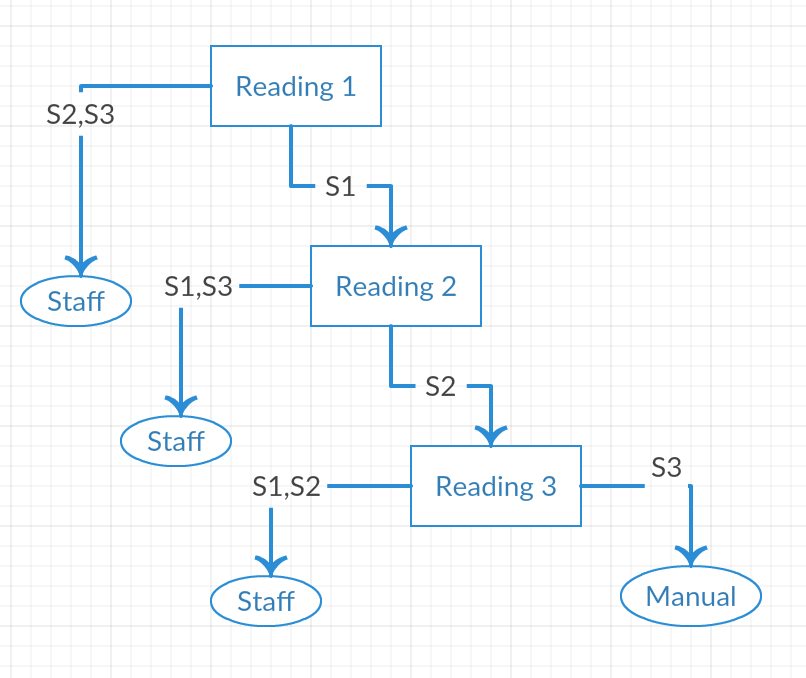
\includegraphics[scale=0.5]{Pictures/dectree.png}
    \caption{Example of a decision tree that classifies the probability of an address being "Staff" or "Manual"}
    \label{fig:dectree}
\end{figure}

In order to learn a decision tree, a splitting condition must be found. The algorithm does this by calculating the expected entropy for each condition and picking the lowest one, thus maximising information gain. \cite{tdndectrees}\\

\par
We first calculate the entropy for each potential condition using
\begin{align*}
	Entropy(S) = -\sum_c p_{(c)} \log_2p_{(c)}
\end{align*}

where $p_{(c)}$ is the frequency of examples of class c in S

%TODO example with table and calculations of entropy


% BEGIN RESULT EVAL %

\section{Evaluating the results}

The methodology is as follows: In the seven days of data, we have
\begin{itemize}
	\item manual - 3574 addresses 
	\item staff - 8045 addresses
	\item no-q - 1633 addresses
	\item privium - 278 addresses
\end{itemize}

Training and testing will be done on a 66\%/34\% train/test split on the whole dataset. We will thus create the tables

\begin{itemize}
	\item train - 8930 addresses 
	\item test  - 4600 addresses
\end{itemize}

The model is trained using the train dataset, then the testing dataset is evaluated using the trained model. Afterwards we compare the predicted labels with the true labels and create the resulting confusion matrix below, that breaks down the performance of the model:


\begin{figure}[H]
    \centering
    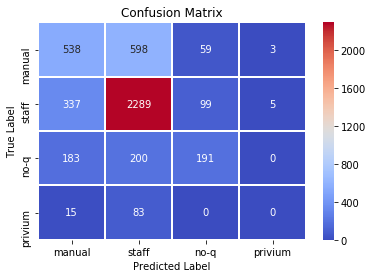
\includegraphics[width=.5\textwidth]{Pictures/decision_tree_confusion.png}
    \caption{Decision tree results (confusion matrix)}
    \label{fig:dectrees:confusion_matrix}
\end{figure}

\subsection{Performance summary}

As described in \ref{section:performance_metrics}, below is the performance summary for decision trees on our data, derived from the confusion matrix in Figure \ref{fig:dectrees:confusion_matrix}. 

\begin{table}[H]
    \centering 
    \begin{tabular}{c|c|c|c|}
        \cline{2-4}
                                                     & \textbf{Precision} & \textbf{Recall} & \textbf{Examples} \\ \hline
        \multicolumn{1}{|l|}{\textbf{manual}}        & 0.50               & 0.45            & 1198              \\ \hline
        \multicolumn{1}{|l|}{\textbf{staff}}         & 0.72               & 0.84            & 2730              \\ \hline
        \multicolumn{1}{|l|}{\textbf{no-q}}          & 0.55               & 0.33            & 574               \\ \hline
        \multicolumn{1}{|l|}{\textbf{privium}}       & 0.00               & 0.00            & 98                \\ 
        \hline \hline
        \multicolumn{1}{|l|}{\textbf{Average / Total}} & 0.44               & 0.40            & 4600               \\ 
        \hline \hline
        \multicolumn{1}{|l|}{\textbf{Accuracy}}      & \multicolumn{3}{c|}{0.66}                                \\ \hline
    \end{tabular}   
    \caption{Performance summary for decision trees}
\end{table}
\subsection{Interpretation and Conclusion}
This approach has yielded far better results than label propagation did, but its accuracy is still unsatisfactory. The reason for this is mostly due to inconsistencies in readings, with many parameters affecting signal strengths: other people, location of the Bluetooth device, owner's rotation, etc. In the end, the difference between keeping the device in the left or right pocket might be interpreted differently by our algorithm due to the line of sight to the different sensors, and this could potentially have an impact on the results. \par
\medskip
Another effect of this is that it is difficult to line the timelines up. A device might be picked up by a sensor far before another one, so their timelines, although similar, will be offset. This is incompatible with the current approach, where, ideally, we hope all devices to be in the same spot at $t_0$.\par
\medskip
We have therefore decided that decision trees are not the way to go either, and will continue trying to find other algorithms that can learn to ignore such irregularities.
\chapter{Convolutional Neural Networks}\label{chap:CNN}
\section{Basic Neural networks}\label{section:neural}
Neural networks, in their basic form of feed-forward neural networks are structures of hierarchical nodes (neurons or units) organised in layers, that can be used for machine learning problems, including classification. 

\par
In neural networks, the first layer represents the input features and the last layer the output features (e.g. classified labels or predicted values). The layers in between input and output are called hidden layers, as they represent hidden features in the data, which can be learned.

\begin{figure}[H]
    \centering
    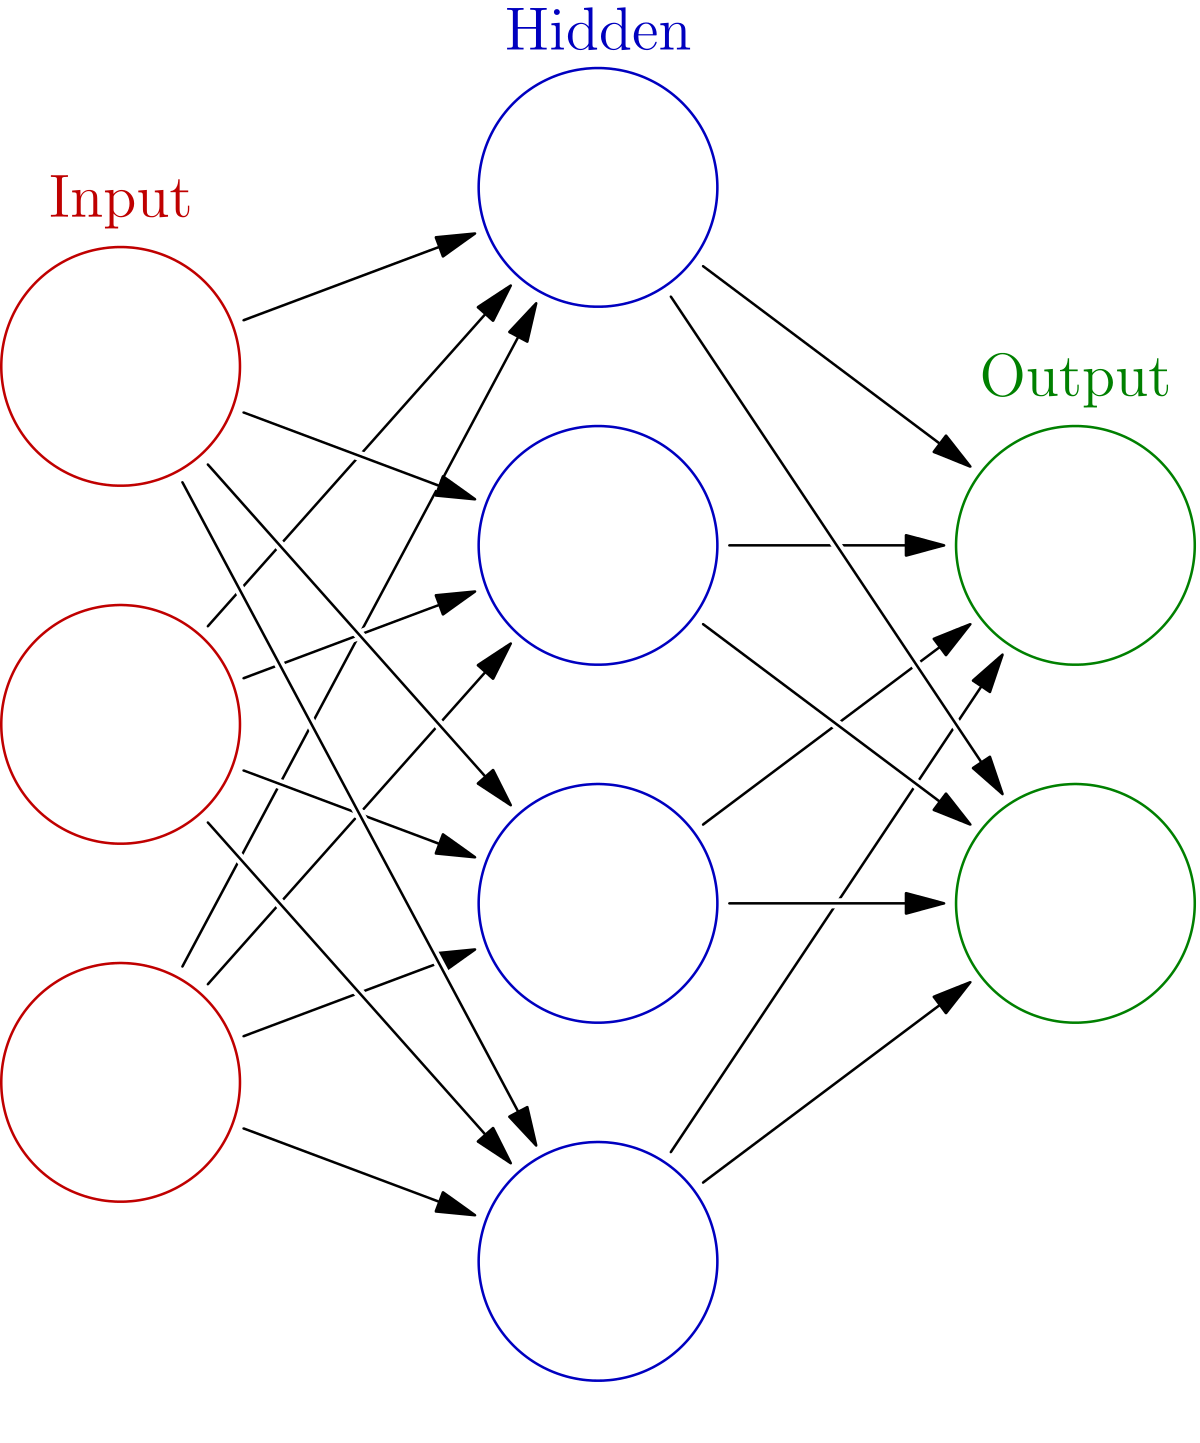
\includegraphics[width=0.35\textwidth]{Pictures/neural_network.png}
    \caption{Example of a basic feed-forward neural network}
    \label{fig:neural_network}
\end{figure}

\par
The layers in a neural network are fully connected, meaning every unit in a given layer is connected to every unit in the next layer, while each link between nodes is assigned a weight. The values of input features propagate forward through the network to the output nodes, as each unit's output is a function of the the weighted sum of inputs. We can generally define any unit's output (activation) as the following \cite{nielsenneural}:
\begin{equation*}
     a^{l}_j = \sigma\left( \sum_k w^{l}_{jk} a^{l-1}_k + b^l_j \right) 
     \label{eq:neuron_output}
\end{equation*}
where:
\begin{itemize}
    \item $a_j^l$ is the output of the $j$-th neuron in the $l$-th layer of a neural network
    \item $a_k^{l-1}$ is the output of the $k$-th neuron in the layer preceding the $l$-th layer ($l-1$)
    \item $w_{jk}^l$ is the weight of the $k$-th neuron in the previous layer ($l-1$) with respect to the $j$-th neuron in the $l$-th layer
    \item $b_j^l$ is the output of the $j$-th bias neuron in the $l$-th layer of the network
    \item $\sigma$ is an activation function
\end{itemize}

\subsection{Activation functions}
\label{sec:activation_functions}
Activation functions are used to influence the propagation of values in a neural network, as they define the outputs of nodes. Several different functions can be used and their effectiveness generally depends on properties such as differentiability and efficiency of computation, which can influence the performance of a neural network during back-propagation (process of approximating optimal weights using e.g. stochastic gradient descent). We will define two main functions that we will use later in the report: \textit{ReLU} and \textit{Softmax}.

\subsubsection{ReLU (Rectified Linear Unit)}
ReLU (Rectified Linear Unit) is a typical activation function used in deep neural networks due to its simplicity and and computational efficiency. It is defined as:
\begin{equation*}
    relu(x) = 
    \begin{cases}
        0,  & \text{if } x < 0\\
        x,  & \text{if } x \geq 0
    \end{cases}
\end{equation*}
It has been shown that, for example in convolutional neural networks, training time can improve as much as six times when using ReLU compared to previously favoured activation functions.\cite{krizhevsky2012imagenet}

\subsubsection{Softmax}
\label{sec:softmax}
The softmax function is a function that can be used in the output layers of neural networks. More specifically, it is generally used as the output activation function in multi-label classification problems in order to generate a proper probability distribution for the labels. It is defined as:
\begin{equation*}
    softmax(y_i) = \frac{e^{y_i}}{\sum_{j} e^{y_j}}
\end{equation*}
where $y$ is a vector of inputs and $y_i$ its $i$-th element

\subsection{Learning \& back-propagation}
In order to be able to classify examples using a neural network, the network has to be trained with a training data set. The goal of training a neural network is to \textit{learn} (approximate) the optimal weights the network should use in order to accurately classify data based on input. This approximation of optimal weights is facilitated by the back-propagation algorithm:
\medskip
\par
In the beginning of training, all the weights are randomly initialised. Then, for each example from the training set, the following operations are performed:
\begin{enumerate}
    \item Forward-propagate the values from the input layer ($a^1$), through hidden layers ($a^2$ to $a^{L-1}$) until the output layer values are obtained ($a^L$ where $L$ is the number of layers in the network). This can be calculated using \cref{eq:neuron_output}.
    
    \item Calculate the total error, using a cost function $C$, given each output layer value $a^L_k$ and its corresponding ground truth value (the target) $t_k$.
    
    \item Back-propagate the total error from the output layer ($L$) through hidden layers ($L-1$ until $2$) to the input layer ($1$). During back-propagation, the effect of weights on the cost $C$ is being approximated. For a given weight, this can be mathematically expressed for a node $a^l_j$ as the following partial derivative of $C$ \cite{nielsenneural}:
    \begin{equation*}
        \frac{\partial C}{\partial w^l_{jk}} = a^{l-1}_k \cdot \delta^l_j
    \end{equation*}
    where
    \begin{itemize}
        \item $C$ is the cost function
        \item $w^l_{jk}$ is the weight of the $k$-th neuron in layer $l-1$ with respect to the $j$-th neuron in layer $l$
        \item $a^{l-1}_k$ is the output (activation) of the $k$-th neuron in layer $l-1$
        \item $\delta^l_j$ is an \textit{error term} that can be derived based on the specific cost and activation functions used in the network
    \end{itemize}
    
    \item For each weight $w^l_{jk}$, update the weight according to the following assignment\cite{nielsenneural}\cite{thomas_nn_slides}:
    \begin{equation*}
        w^l_{jk} := w^l_{jk} + \eta \cdot \delta^l_j \cdot a^{l-1}_k
    \end{equation*}
    where $\eta$ is a constant factor called learning rate.
\end{enumerate}

\par
In summary, during training, batches of training examples are being fed through the network. Back-propagation is used in order to compute the gradient of the cost function $\nabla C$, based on the error between the predicted outputs and the true outputs. Then, given $\nabla C$, the network weights can be optimised for to minimise the cost, by changing them in the opposite direction of $\nabla C$. This optimisation technique, formally known as gradient descent, is what facilitates the \textit{learning} in a neural network.

\subsection{Cost function}
A cost function (also known as error or loss function) facilitates the measurement of error, given the network output and the ground truth. As described earlier, the value of the function serves as a performance metric during training and influences the weight adjustments.
\medskip
\par
\subsubsection{Cross-entropy}
The cost function that will be used in our experiments is called cross-entropy, and can be defined as \cite{nielsenneural}:
\begin{equation*}
    C = - \sum_i y_i \cdot \log(p_i)
\end{equation*}
where:
\begin{itemize}
    \item $y_i$ is the ground truth value for the $i$-th output
    \item $p_i$ is the $i$-th predicted value, corresponding to the output (activation) of the $i$-th neuron in the output layer of the network
    \item $\log$ is the natural logarithm ($\log_e$)
\end{itemize}
\medskip
\par
As mentioned earlier, our problem is that of multi-label classification and therefore our neural network output should be a probability distribution over the different classes (hence the usage of the softmax activation function in the output layer, as per \cref{sec:softmax}).
\medskip
\par
Cross-entropy is a commonly used cost function in multiple fields, when it comes to optimisation of probability distributions. In deep neural networks specifically, cross-entropy is often leveraged for the nature of its derivative, which avoids slowdown during learning.






\pagebreak
\section{Convolutional Neural Networks}

\par
Convolutional neural network (CNN) represents a deep learning model that can be used in classification problems. It can be defined as a special category of neural networks which replace the general matrix multiplication with convolutions in at least one layer of the structure.\cite{Goodfellow}
CNN is commonly used for data that follow some patterns. Complex patterns can be identified starting with simple ones in the first convolution layers. Examples of applications using CNN are: human digit recognition \cite{digits}, human activity recognition \cite{convolutional} or image classification. The input data is usually represented in the shape of a grid, but the performance is also good with 1-dimensional data.

\subsection{Convolution, mathematical concept}
\par
The intuition behind the convolutions has the bases in mathematics where the convolution of two function $f(t)$ and $g(t)$  \cite{Goodfellow} is denoted by:
\begin{equation*}
    (f*g)(t) = \int_{-\infty}^{\infty}f(\tau)g(t-\tau) d\tau
\end{equation*}

\begin{figure}[H]
    \centering
    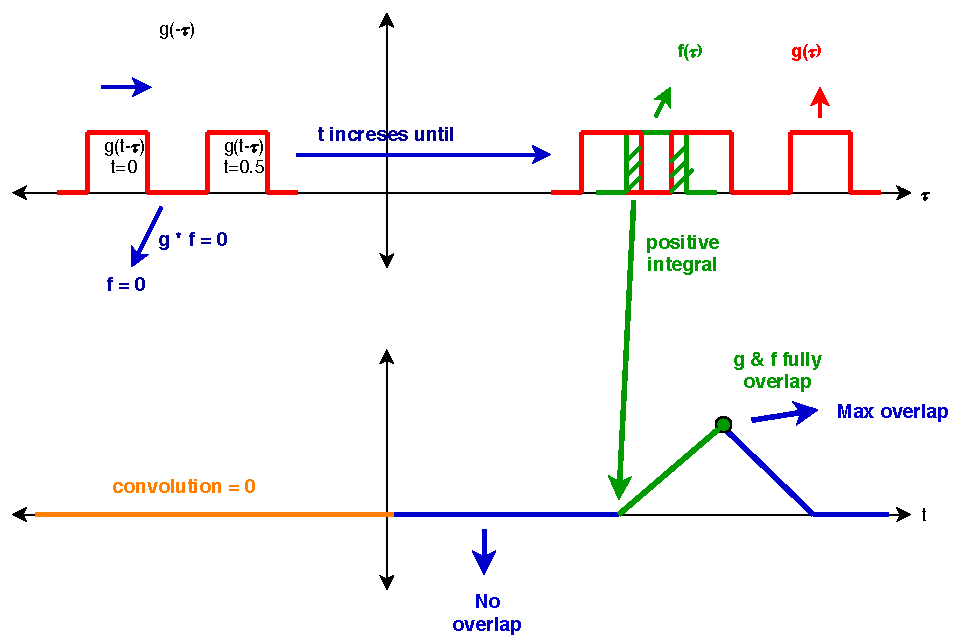
\includegraphics[width=0.8\textwidth]{convolutionMath}
    \caption{Graphical mathematical example of convolution}
    \label{fig:convolutionMath}
\end{figure}

\par
Using \cref{fig:convolutionMath} the convolution is explained as follows:
\begin{enumerate}
    \item take two functions: $f(\tau)$ and $g(\tau)$ 
	\item let then consider $g(-\tau)$, in this case f=0 and the result of $(f*g)(t) = 0$ \cref{fig:convolutionMath}
	\item sweeping $g(-\tau)$ across the domain, from $(-\infty)$ to 0, the result will remain 0 due to f = 0
	\item when $g$ starts to overlap $f$, the integral = positive value
	\item when the two functions are fully overlapped, the integral reaches the maximum value
	\item after this point g will continue to sweep across f, but the overlap zone will decrease; the value for the integral will also start to decrease until it reaches 0 again (the point where there is no more overlapping)
\end{enumerate}
 
To summarise, the convolution defined as $(f*g)(t)$ tell us the degree to which f and g overlap at t as g sweeps across the domain at t.

\subsection{CNN architecture}
\par
The CNN structure consists of an input layer, one or more hidden layers from which at least one must be a convolution layer, and the output layer. The number of layers is dependent on the problem that needs to be solved. The deeper the network is, the more complex patterns can be identified by the convolutional neural network. 
For a better understanding of a structure we will use an example of image classification.

\subsubsection{Input}
\par
The input represents data used to feed the network. It can take several shapes in terms of the size (1D, 2D, 3D). Pictures for example, can be represented by a 2D matrix where the filled pixels will have value 1 and the others 0.
\cref{fig:input} describes the transformation from an image to a 7x7 matrix input.

\begin{figure}[ht]
    \centering
    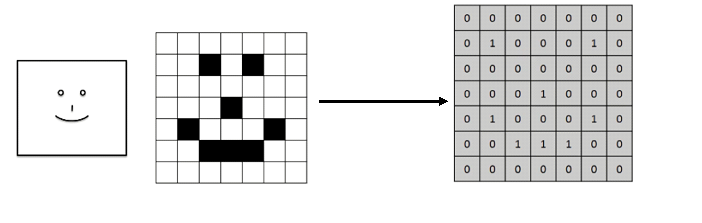
\includegraphics[width=0.9\textwidth]{CNNinput}
    \caption{Graphical example of a input}
    \label{fig:input}
\end{figure}

\subsubsection{Convolution layer}
\label{sec:convolution layer}
\par
A convolution layer has three elements: an input, one or more feature detectors( filters) and an output (feature map) which will serve as input for the next layer. Based on the number of filters defined, there can be learnt as many features as we want in a single layer.\newline
\par
A feature detector convolves the given input, searching for patterns. It has a size denoted also as kernel size. In \cref{fig:convolution} the size is set to 3x3. 

\begin{figure}[ht]
    \centering
    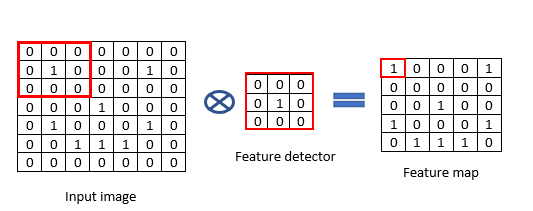
\includegraphics[width=0.9\textwidth]{convolutionLayer}
    \caption{Graphical example of a convolution layer}
    \label{fig:convolution}
\end{figure}

\begin{figure}[ht]
    \centering
    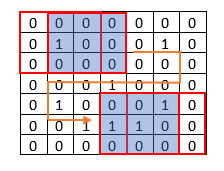
\includegraphics[width=0.5\textwidth]{filter}
    \caption{Graphical example of filter sliding}
    \label{fig:filter}
\end{figure}

\par
\cref{fig:convolution} and \cref{fig:filter} represent graphical representation of how convolution works. The steps are as follows:
\begin{enumerate}
    \item define the feature detector; let's assume that for the given example we first want to find features like an eye or the nose of the smiley face; those are represented by a single filled pixel or a value of 1 in the input matrix; the chosen filter will convolute the input to find the feature
    \item place the filter in the top-left-corner of the input
    \item compute an element-wise product between the defined filter and input matching cells
    \item store the result in the convolution layer output called feature  map as in \cref{fig:convolution}
    \item move the filter to the next column and repeat 3 and 4
    \item the filter will be sliding through all the input until it reaches the right bottom corner (\cref{fig:filter}); the filter will be moved one column at time. This movement is also called stride
    \item the feature map resulted will be the input for the next network layer
\end{enumerate}

\subsubsection{Activation layer}
\par
Another layer type that is often found in CNNs after a convolution layer is an \textit{activation} layer. The neurons of this layer use an activation function (as defined in \cref{sec:activation_functions}) in order to introduce non-linearity into the model. This process is sometimes also considered as simply part of the convolution operation.

\subsubsection{Pooling}
\label{sec:pooling layer}
\par 
The concept of pooling plays an important role in convolution neural networks, allowing the recognition of an image independently of the spatial position and also reducing the size on the input.
With our example of the smiley face the network needs to be able to correctly classify the image disregarding the position \cref{fig:positions}.

\begin{figure}[ht]
    \centering
    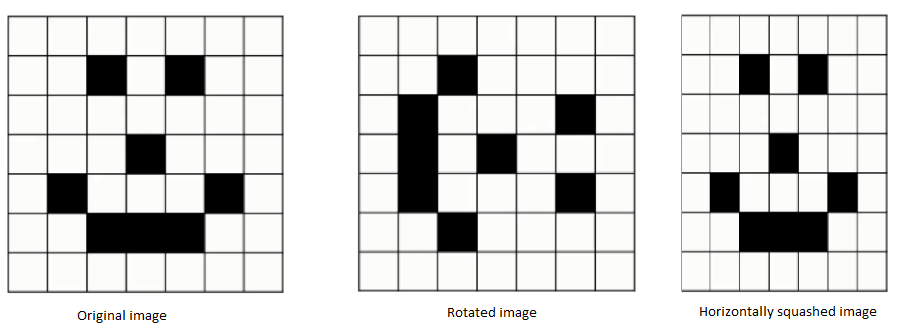
\includegraphics[width=0.8\textwidth]{smileyFacePosition}
    \caption{Graphical example of image positions}
    \label{fig:positions}
\end{figure}

\par
Pooling can be chosen differently from the existing several types according with the problem. Some of the existing types are:
\begin{itemize}
    \item max pooling
    \item min pooling
    \item mean pooling
\end{itemize}

\par
The max pooling concept it is using the feature map as input and outputs a pooled feature map. It is working based on the following steps and \cref{fig:pooling}:

\begin{figure}[H]
    \centering
    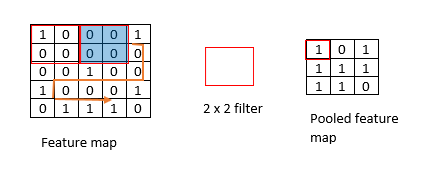
\includegraphics[width=0.8\textwidth]{maxPooling}
    \caption{Graphical example of max pooling}
    \label{fig:pooling}
\end{figure}

\begin{enumerate}
    \item define the size of the filter that will be used
    \item place the filter on top left corner of the feature map
    \item pick the maximum value from the selected region
    \item start from the top left corner and insert the selected value  
    \item define the stride value, in \cref{fig:pooling}, stride = 2
    \item move the filter along the feature map based on the stride value, and repeat 3
    \item move through the pooled feature map as the filter moves and insert the max value
\end{enumerate}
\par
The principle of min pooling or mean pooling is the same except for the way of choosing the value from the selected area. In other words, it can also be the minimum value or the mean value.\newline


\subsubsection{Fully connected layer}
\par 
A fully connected layer is a typical layer used in basic neural networks where each neuron in layer ($l$) is connected to each neuron in layer ($l-1$), as illustrated in \cref{fig:neural_network} and defined in \cref{eq:neuron_output}.

\subsubsection{Output}
\par 
The output consists of neurons where the number can vary based on the classification type (one class or multiple classes). The output of each neuron is the network's belief that the input belongs to said class. %network outputs a value interpreted as how much the network believes the input belongs to a certain class. 

\pagebreak
\section{Implementation}
\subsection{Input model}

\par
In order to utilise Convolutional Neural Network (CNN) for passenger classification, we must first decide on the nature of the input. To represent a mobile device, we can follow the steps of modelling the data defined in chapter 5. We define table $T$ to have size:

\begin{align*}
    |S| \times t_m
\end{align*}

\par
where:
\begin{itemize}
	\item $S$ is the set of sensors installed in the airport’s arrival gate
	\item $t_m$ is the maximum time stamp
\end{itemize}

\par
The size of $T$ now depends on the number of sensors that measured mobile device and number of seconds that elapsed between first and last measurement. The table size, therefore, varies for each mobile device. To use CNN, we must first reshape each mobile device table to a fixed size. We selected all 13 sensors located in the arrival gate (see \cref{fig:stat:readingspersensor}) and first 45 minutes (2700 seconds) of measurements. Figure \ref{fig:stat:timespentdistbylabel} shows that 45 minutes is a reasonable threshold - after we average the ratios per label, only $5.4\%$ of mobile devices remain in the arrival gate area longer. We define a fixed size of $13 \times 2700$ and minimum signal strength -75. We then follow the steps described in chapter 5 in order to obtain table $T$. Table $T$ now looks as following:

\begin{table}[H]
    \centering
    \begin{tabular}{|l|l|l|l|l|}
    \hline
    t    & S1  & S2  & ... & S13 \\ \hline
    0    & -70 & -75 & ... & -75 \\ \hline
    1    & -65 & -75 & ... & -70 \\ \hline
    2    & -60 & -75 & ... & -68 \\ \hline
    3    & -60 & -75 & ... & -65 \\ \hline
    4    & -50 & -75 & ... & -63 \\ \hline
    5    & -40 & -75 & ... & -60 \\ \hline
    ...  & ... & ... & ... & ... \\ \hline
    2696 & -60 & -75 & ... & -75 \\ \hline
    2697 & -75 & -75 & ... & -75 \\ \hline
    2698 & -75 & -75 & ... & -75 \\ \hline
    2699 & -75 & -75 & ... & -75 \\ \hline
    \end{tabular}
    \caption{Input table T}
\end{table}

\par
We then map each signal strength value t in the table from interval $[a, b] (a = -75, b = -3)$ to $[a', b'] (a' = 0, b' = 100)$. We do this, because we use Rectified linear unit (ReLU) as activation function in the activation layer of CNN, which returns zero on any negative input. We used the following function for mapping the signal strengths:

\begin{align*}
     f(t) =  a' +  \big( \frac{b' - a'}{b - a} \big) * (t-a), a \neq b  
\end{align*}

\par
Where:
\begin{itemize}
    \item $t$ is the signal strength
	\item $a$ is the lowest measured signal strength
	\item $b$ is the highest measured signal strength
\end{itemize}

\par
We can now apply function f to each value in the table $T$:

\begin{align*}
     T_{p_{i,j}} = f(T_{i,j})  
\end{align*}

\par
Where:
\begin{itemize}
	\item $T_{i,j}$ is the value in the  $i^{th}$  row and $j^{th}$ column of table $T$
	\item $T_{p_{i,j}}$ is the value in the $i^{th}$ row and $j^{th}$ column of table $T_p$
\end{itemize}

\par
The table $T_p$ can be represented as a matrix $P$, which we can use as an input for the convolutional neural network:

\begin{align*}
        P = 
        \begin{bmatrix}
            6.94     & 0        & \cdots & 0        \\
            13.89    & 0        & \cdots & 6.94     \\
            20.83    & 0        & \cdots & 9.72     \\
            20.83    & 0        & \cdots & 13.89    \\
            \vdots   & \vdots   & \ddots & \vdots   \\
            20.83    & 0        & \cdots & 0        \\
            0        & 0        & \cdots & 0        \\
            0        & 0        & \cdots & 0        
        \end{bmatrix}
\end{align*}

\subsection{Design}
\label{sec:cnn:design}

\par 
The Convolutional neural network consists of convolutional, pooling, activation and fully connected layers. Fig \ref{fig:cnn:design1} shows how the input matrix $P$ flows through convolutional, pooling and activation layers. The output of the last activation layer is then flattened into a layer of neurons, as shown on Fig \ref{fig:cnn:design2}.

\begin{figure}[H]
    \centering
    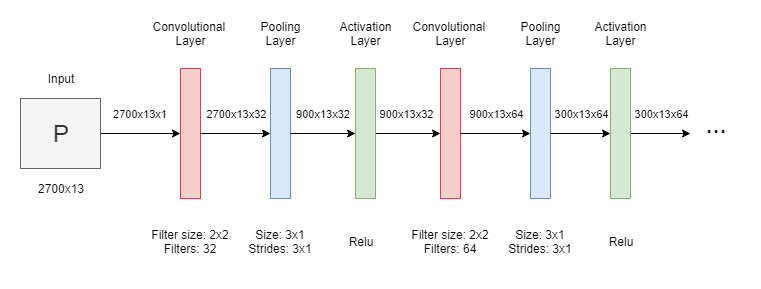
\includegraphics[width=.9\textwidth]{Pictures/Cnn_design1.png}
    \caption{CNN Flow chart 1}
    \label{fig:cnn:design1}
\end{figure}

\begin{figure}[H]
    \centering
    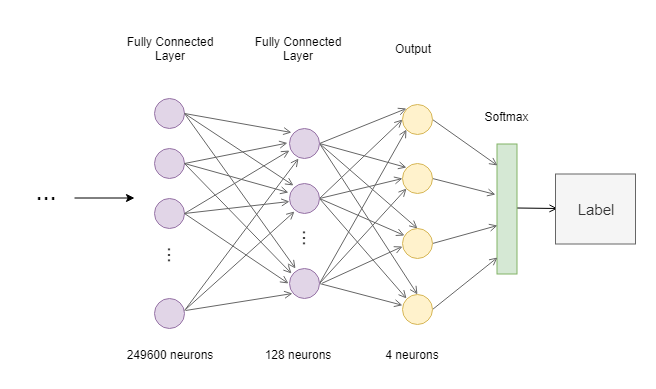
\includegraphics[width=.9\textwidth]{Pictures/Cnn_design2.png}
    \caption{CNN Flow chart 2}
    \label{fig:cnn:design2}
\end{figure}

\par
The first convolutional layer takes a single matrix $P$ as an input. It creates 32 filters of size $2 \times 2$ and each filter convolves over $P$ (as described in section \ref{sec:convolution layer}) without skipping any rows and columns. Each filter outputs its own convoluted matrix, therefore the output of the first convolutional layer has 32 channels. The dimensions of the all output matrices remain the same as dimensions of $P$. The layer output can defined as follows:

\begin{align*}
     P_{1} = 2700 \times 13 \times 32 
\end{align*}

\par
The first pooling layer takes the output $P_{1}$ and down-samples it with a $3 \times 1$ filter (as described in section \ref{sec:pooling layer}). This filter is applied to every sub-region of every input matrix. The output of this layer can be defined as follows:

\begin{align*}
     P_{2} = 900 \times 13 \times 32 
\end{align*}

\par
The output $P_{2}$ is then passed through an activation layer. This layer uses the Rectified linear unit activation function, which ensures that any negative value in the input matrices is set to 0. The dimensions of the output do not change:

\begin{align*}
     P_{3} = P_{2} 
\end{align*}

\par 
The second convolutional layer takes an input P3 and creates 64 filters of size $2 \times 2$. The output of this layer has 64 channels and dimensionality of each input matrix remains the same. The output of this layer can be defined as follows:

\begin{align*}
     P_{4} = 900 \times 13 \times 64
\end{align*}

\par
The second pooling takes and input P4 and down-samples it with a $3 \times 3$ filter. The output of this layer can be defined as follows:

\begin{align*}
     P_{5} = 300 \times 13 \times 64
\end{align*}

\par
As before, the next activation layer applies the Rectified linear unit activation function. The dimensions of the output do not change:

\begin{align*}
     P_{6} = P_{5} 
\end{align*}

\par 
The output $P_{6}$ is then flattened into one layer of neurons. The number of neurons of the first fully connected layer can be calculated by multiplying all dimensions of the output  $P_{6}$, which is equal to 249600 neurons. These neurons are then connected to the second fully connected layer, which contains 128 neurons. The output layer then estimates how likely it is that the input image belongs to each of the 4 labels – manual, staff, no queue and privium.

\par 
To normalise the output values, we use the softmax function, which ensures that each label value is between 0 and 1, and that all 4 labels sum to 1, representing the probability distribution of the labels. The argmax function then selects the largest probability, which corresponds to the predicted label.

\subsection{Evaluation}

\par 
We selected all mobile addresses from the seven days of data measured from $6^{th}$ to $12^{th}$ September 2018. We used 13530 unique addresses distributed as follows:

\begin{itemize}
	\item manual - 3574 addresses
	\item staff - 8045 addresses
	\item no-q - 1633 addresses
	\item privium - 278 addresses
\end{itemize}

\par
The CNN model was configured according to the network design in \cref{sec:cnn:design}, alongside with the following hyper-parameters: 
\begin{itemize}
	\item number of training examples - 9065
	\item number of testing examples - 4465
	\item learning rate - 0.0001 ($10^{-4}$)
	\item batch size - 16
	\item number of optimisation iterations - 1000
	\item number of epochs - 1
\end{itemize}

\par
The CNN model was trained on two thirds of addresses, such that two thirds of addresses were randomly selected from each label. Testing set consisted of the remaining third, distributed as follows:

\begin{itemize}
	\item manual - 1179 addresses
	\item staff - 2655 addresses
	\item no-q - 539 addresses
	\item privium - 92 addresses
\end{itemize}

\par
The following confusion matrix breaks down the performance of this model:

\begin{figure}[H]
    \centering
    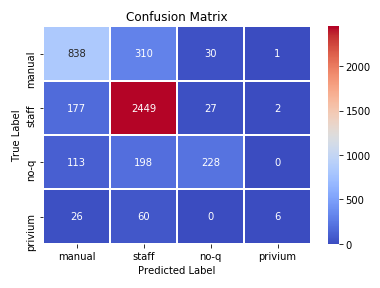
\includegraphics[width=.5\textwidth]{Pictures/Cnn_cm2.png}
    \caption{CNN results (Confusion matrix)}
    \label{fig:cnn:cm}
\end{figure}

\par
As described in \ref{section:performance_metrics}, the following is the performance summary of CNN derived from the confusion matrix above:

\begin{table}[H]
    \centering
    \begin{tabular}{|l|c|c|c|}
    \hline
                            & \textbf{Precision} & \textbf{Recall} & \textbf{Examples} \\ \hline
    \textbf{manual}         & 0.73               & 0.71            & 1179               \\ \hline
    \textbf{staff}          & 0.81               & 0.92            & 2655               \\ \hline
    \textbf{no-q}           & 0.80               & 0.42            & 539                \\ \hline
    \textbf{privium}        & 0.67               & 0.07            & 92                 \\ \hline
    \textbf{Average/ Total} & 0.7525             & 0.53           & 4465              \\ \hline
    \textbf{Accuracy}       & \multicolumn{3}{c|}{78.9}                                \\ \hline
    \end{tabular}
    \caption{Performance summary for CNN}
\end{table}

\pagebreak
\section{Interpretation and Conclusion}

\par
The overall accuracy of this model was considerably higher compared to other previously utilised models. The model itself performed the worst when it comes to classification of privium and no-q passengers. This could be due to small number of examples in the data-set for both labels. On the other hand we can conclude that the model performs a lot better with classification of manual passengers and staff members, which are the most common types of mobile devices detected at the arrival gate. 
\chapter{Conclusion}\label{chap:results}
\section{Results}
Throughout this project we have shown that it is possible to streamline the classification process of Blip Systems using machine learning techniques, thus reducing and potentially eliminating the need for their data calibration and modelling steps, as described by fig \ref{fig:strategy_of_blip}. We have explored three different machine learning models, respectively label propagation, decision trees and convolutional neural networks with varying degrees of success. 
\par
\medskip
Our first attempt was using a label propagation algorithm which required a similarity function to compare two different mobile addresses. We did this by modelling the data as a multidimensional time series that we could then compute similarities on. This yielded the worst results for us due to the large inconsistencies in data between equally labelled instances. Label propagation therefore was only able to categorise our data with an abysmal 36\% accuracy.
\par
\medskip
We followed that up by changing the data model so that we represented each mobile device by a series of the closest perceived sensors, therefore creating a virtual path for the device. Using a logarithmic time scale enabled us to retain important information while simultaneously reducing rare, disproportionately long instances. We were then able to train a decision tree on the data, yielding a much improved 66\% accuracy. 
\par
\medskip
Finally we adapted the model yet again so that we were left with fixed-size bi-dimensional matrices for each device, representing the multidimensional time series. This we were then able to interpret as a grayscale image, which allowed us to train a convolutional neural network. This resulted in our final and best results, a 79\% accuracy. 

\section{Future work}

In the future, more work can be done on mixing different approaches together. For example, figuring out a way to filter some of the very long series as automatically being staff. Finding a way to filter out the privium class would also be very helpful, since it is the class that has proven the most difficult for us to categorise. Given these findings, we believe there is also potential in combining the resource-intensive approach of Blip Systems together with our machine learning approach. In this scenario, the rules designed by Blip Systems could be used for filtering the instances that have proven to be more problematic in our experiments.
%


%\input{Report/probAnalysis.tex}


\clearpage

%\pagenumbering{gobble}

%Figurliste
\listoffigures

%Tabelliste
\listoftables

%Litteraturliste
\bibliography{literature}

%Bilag___APENDICE
%\input{Bilag/bilag.tex}
	
\end{document}
